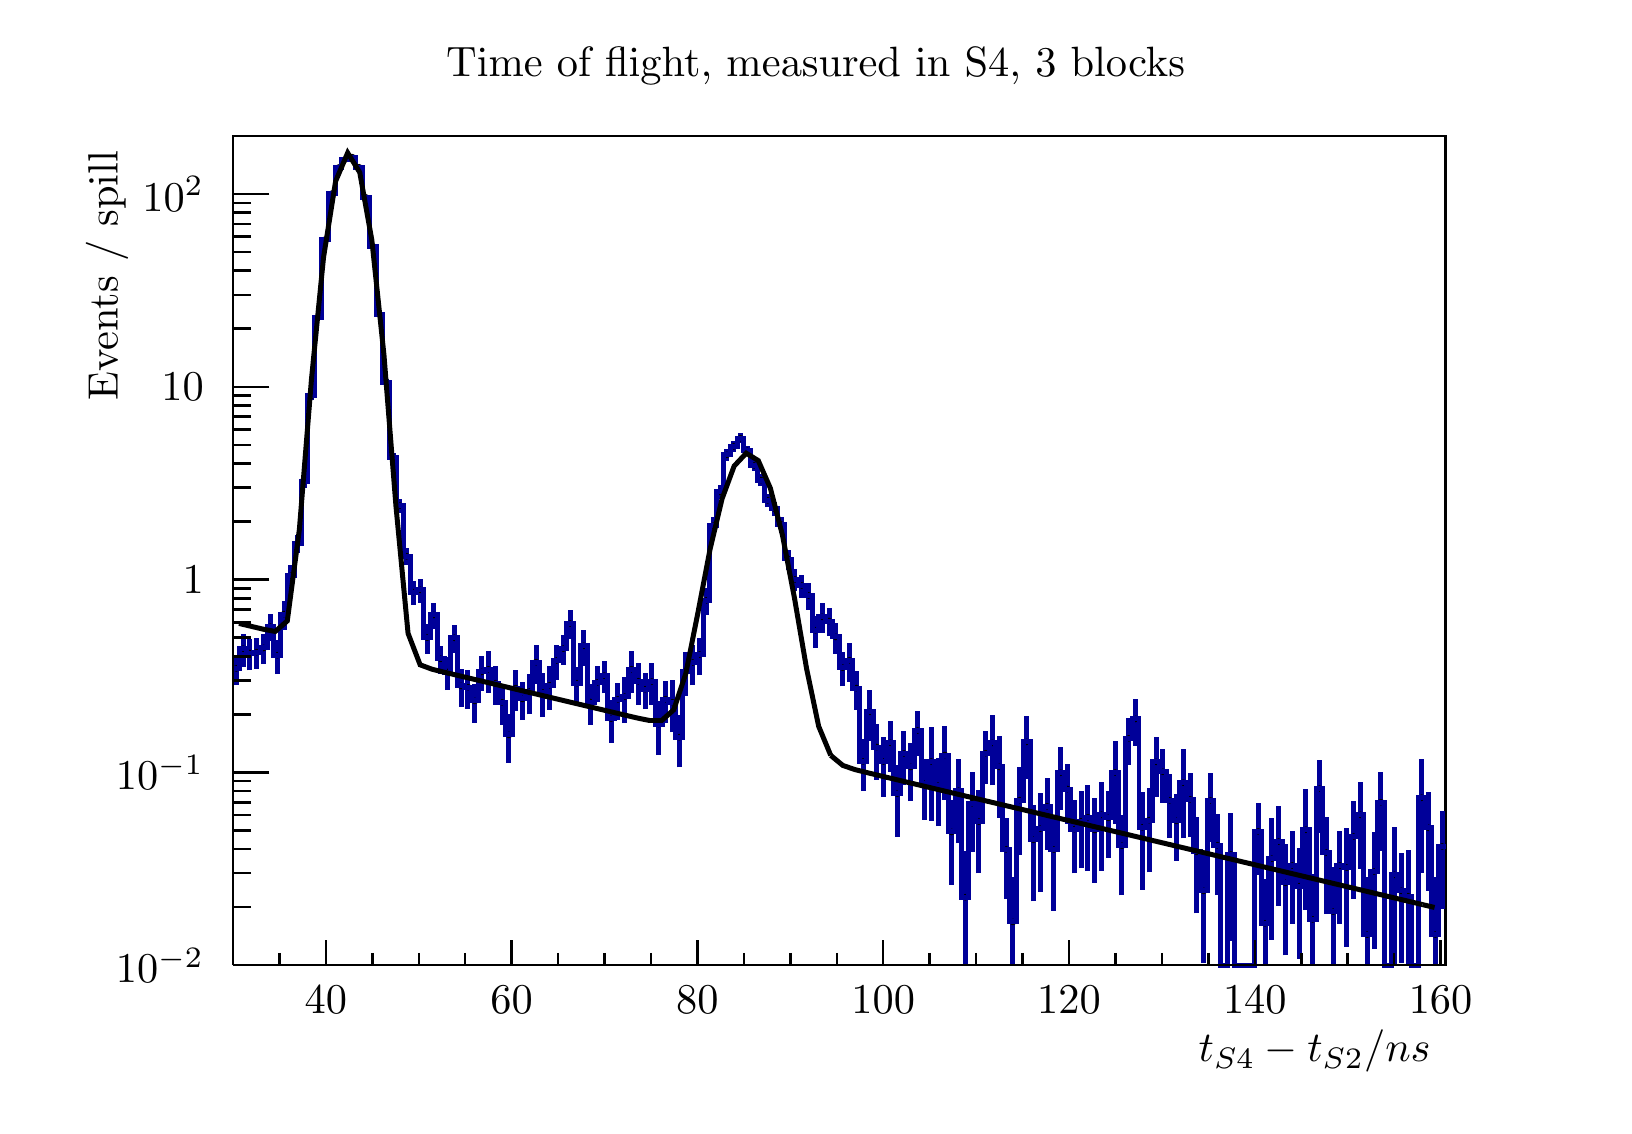
\begin{tikzpicture}
\pgfdeclareplotmark{cross} {
\pgfpathmoveto{\pgfpoint{-0.3\pgfplotmarksize}{\pgfplotmarksize}}
\pgfpathlineto{\pgfpoint{+0.3\pgfplotmarksize}{\pgfplotmarksize}}
\pgfpathlineto{\pgfpoint{+0.3\pgfplotmarksize}{0.3\pgfplotmarksize}}
\pgfpathlineto{\pgfpoint{+1\pgfplotmarksize}{0.3\pgfplotmarksize}}
\pgfpathlineto{\pgfpoint{+1\pgfplotmarksize}{-0.3\pgfplotmarksize}}
\pgfpathlineto{\pgfpoint{+0.3\pgfplotmarksize}{-0.3\pgfplotmarksize}}
\pgfpathlineto{\pgfpoint{+0.3\pgfplotmarksize}{-1.\pgfplotmarksize}}
\pgfpathlineto{\pgfpoint{-0.3\pgfplotmarksize}{-1.\pgfplotmarksize}}
\pgfpathlineto{\pgfpoint{-0.3\pgfplotmarksize}{-0.3\pgfplotmarksize}}
\pgfpathlineto{\pgfpoint{-1.\pgfplotmarksize}{-0.3\pgfplotmarksize}}
\pgfpathlineto{\pgfpoint{-1.\pgfplotmarksize}{0.3\pgfplotmarksize}}
\pgfpathlineto{\pgfpoint{-0.3\pgfplotmarksize}{0.3\pgfplotmarksize}}
\pgfpathclose
\pgfusepathqstroke
}
\pgfdeclareplotmark{cross*} {
\pgfpathmoveto{\pgfpoint{-0.3\pgfplotmarksize}{\pgfplotmarksize}}
\pgfpathlineto{\pgfpoint{+0.3\pgfplotmarksize}{\pgfplotmarksize}}
\pgfpathlineto{\pgfpoint{+0.3\pgfplotmarksize}{0.3\pgfplotmarksize}}
\pgfpathlineto{\pgfpoint{+1\pgfplotmarksize}{0.3\pgfplotmarksize}}
\pgfpathlineto{\pgfpoint{+1\pgfplotmarksize}{-0.3\pgfplotmarksize}}
\pgfpathlineto{\pgfpoint{+0.3\pgfplotmarksize}{-0.3\pgfplotmarksize}}
\pgfpathlineto{\pgfpoint{+0.3\pgfplotmarksize}{-1.\pgfplotmarksize}}
\pgfpathlineto{\pgfpoint{-0.3\pgfplotmarksize}{-1.\pgfplotmarksize}}
\pgfpathlineto{\pgfpoint{-0.3\pgfplotmarksize}{-0.3\pgfplotmarksize}}
\pgfpathlineto{\pgfpoint{-1.\pgfplotmarksize}{-0.3\pgfplotmarksize}}
\pgfpathlineto{\pgfpoint{-1.\pgfplotmarksize}{0.3\pgfplotmarksize}}
\pgfpathlineto{\pgfpoint{-0.3\pgfplotmarksize}{0.3\pgfplotmarksize}}
\pgfpathclose
\pgfusepathqfillstroke
}
\pgfdeclareplotmark{newstar} {
\pgfpathmoveto{\pgfqpoint{0pt}{\pgfplotmarksize}}
\pgfpathlineto{\pgfqpointpolar{44}{0.5\pgfplotmarksize}}
\pgfpathlineto{\pgfqpointpolar{18}{\pgfplotmarksize}}
\pgfpathlineto{\pgfqpointpolar{-20}{0.5\pgfplotmarksize}}
\pgfpathlineto{\pgfqpointpolar{-54}{\pgfplotmarksize}}
\pgfpathlineto{\pgfqpointpolar{-90}{0.5\pgfplotmarksize}}
\pgfpathlineto{\pgfqpointpolar{234}{\pgfplotmarksize}}
\pgfpathlineto{\pgfqpointpolar{198}{0.5\pgfplotmarksize}}
\pgfpathlineto{\pgfqpointpolar{162}{\pgfplotmarksize}}
\pgfpathlineto{\pgfqpointpolar{134}{0.5\pgfplotmarksize}}
\pgfpathclose
\pgfusepathqstroke
}
\pgfdeclareplotmark{newstar*} {
\pgfpathmoveto{\pgfqpoint{0pt}{\pgfplotmarksize}}
\pgfpathlineto{\pgfqpointpolar{44}{0.5\pgfplotmarksize}}
\pgfpathlineto{\pgfqpointpolar{18}{\pgfplotmarksize}}
\pgfpathlineto{\pgfqpointpolar{-20}{0.5\pgfplotmarksize}}
\pgfpathlineto{\pgfqpointpolar{-54}{\pgfplotmarksize}}
\pgfpathlineto{\pgfqpointpolar{-90}{0.5\pgfplotmarksize}}
\pgfpathlineto{\pgfqpointpolar{234}{\pgfplotmarksize}}
\pgfpathlineto{\pgfqpointpolar{198}{0.5\pgfplotmarksize}}
\pgfpathlineto{\pgfqpointpolar{162}{\pgfplotmarksize}}
\pgfpathlineto{\pgfqpointpolar{134}{0.5\pgfplotmarksize}}
\pgfpathclose
\pgfusepathqfillstroke
}
\definecolor{c}{rgb}{1,1,1};
\draw [color=c, fill=c] (0,0) rectangle (20,13.6782);
\draw [color=c, fill=c] (2.6,1.77816) rectangle (18,12.3103);
\definecolor{c}{rgb}{0,0,0};
\draw [c,line width=0.9] (2.6,1.77816) -- (2.6,12.3103) -- (18,12.3103) -- (18,1.77816) -- (2.6,1.77816);
\definecolor{c}{rgb}{1,1,1};
\draw [color=c, fill=c] (2.6,1.77816) rectangle (18,12.3103);
\definecolor{c}{rgb}{0,0,0};
\draw [c,line width=0.9] (2.6,1.77816) -- (2.6,12.3103) -- (18,12.3103) -- (18,1.77816) -- (2.6,1.77816);
\definecolor{c}{rgb}{0,0,0.6};
\draw [c,line width=1.8] (2.64326,5.33613) -- (2.64326,5.5477);
\draw [c,line width=1.8] (2.64326,5.5477) -- (2.64326,5.72408);
\definecolor{c}{rgb}{0,0,0};
\foreach \P in {(2.64326,5.5477)}{\draw[mark options={color=c,fill=c},mark size=2.402402pt,mark=*,mark size=1pt] plot coordinates {\P};}
\definecolor{c}{rgb}{0,0,0.6};
\draw [c,line width=1.8] (2.72978,5.56414) -- (2.72978,5.79768);
\draw [c,line width=1.8] (2.72978,5.79768) -- (2.72978,5.98906);
\definecolor{c}{rgb}{0,0,0};
\foreach \P in {(2.72978,5.79768)}{\draw[mark options={color=c,fill=c},mark size=2.402402pt,mark=*,mark size=1pt] plot coordinates {\P};}
\definecolor{c}{rgb}{0,0,0.6};
\draw [c,line width=1.8] (2.81629,5.52384) -- (2.81629,5.74333);
\draw [c,line width=1.8] (2.81629,5.74333) -- (2.81629,5.92518);
\definecolor{c}{rgb}{0,0,0};
\foreach \P in {(2.81629,5.74333)}{\draw[mark options={color=c,fill=c},mark size=2.402402pt,mark=*,mark size=1pt] plot coordinates {\P};}
\definecolor{c}{rgb}{0,0,0.6};
\draw [c,line width=1.8] (2.90281,5.54277) -- (2.90281,5.75379);
\draw [c,line width=1.8] (2.90281,5.75379) -- (2.90281,5.92979);
\definecolor{c}{rgb}{0,0,0};
\foreach \P in {(2.90281,5.75379)}{\draw[mark options={color=c,fill=c},mark size=2.402402pt,mark=*,mark size=1pt] plot coordinates {\P};}
\definecolor{c}{rgb}{0,0,0.6};
\draw [c,line width=1.8] (2.98933,5.60077) -- (2.98933,5.80762);
\draw [c,line width=1.8] (2.98933,5.80762) -- (2.98933,5.98072);
\definecolor{c}{rgb}{0,0,0};
\foreach \P in {(2.98933,5.80762)}{\draw[mark options={color=c,fill=c},mark size=2.402402pt,mark=*,mark size=1pt] plot coordinates {\P};}
\definecolor{c}{rgb}{0,0,0.6};
\draw [c,line width=1.8] (3.07584,5.89819) -- (3.07584,6.07841);
\draw [c,line width=1.8] (3.07584,6.07841) -- (3.07584,6.23248);
\definecolor{c}{rgb}{0,0,0};
\foreach \P in {(3.07584,6.07841)}{\draw[mark options={color=c,fill=c},mark size=2.402402pt,mark=*,mark size=1pt] plot coordinates {\P};}
\definecolor{c}{rgb}{0,0,0.6};
\draw [c,line width=1.8] (3.16236,5.47447) -- (3.16236,5.71521);
\draw [c,line width=1.8] (3.16236,5.71521) -- (3.16236,5.91139);
\definecolor{c}{rgb}{0,0,0};
\foreach \P in {(3.16236,5.71521)}{\draw[mark options={color=c,fill=c},mark size=2.402402pt,mark=*,mark size=1pt] plot coordinates {\P};}
\definecolor{c}{rgb}{0,0,0.6};
\draw [c,line width=1.8] (3.24888,6.04112) -- (3.24888,6.23799);
\draw [c,line width=1.8] (3.24888,6.23799) -- (3.24888,6.40405);
\definecolor{c}{rgb}{0,0,0};
\foreach \P in {(3.24888,6.23799)}{\draw[mark options={color=c,fill=c},mark size=2.402402pt,mark=*,mark size=1pt] plot coordinates {\P};}
\definecolor{c}{rgb}{0,0,0.6};
\draw [c,line width=1.8] (3.33539,6.57329) -- (3.33539,6.72391);
\draw [c,line width=1.8] (3.33539,6.72391) -- (3.33539,6.85582);
\definecolor{c}{rgb}{0,0,0};
\foreach \P in {(3.33539,6.72391)}{\draw[mark options={color=c,fill=c},mark size=2.402402pt,mark=*,mark size=1pt] plot coordinates {\P};}
\definecolor{c}{rgb}{0,0,0.6};
\draw [c,line width=1.8] (3.42191,7.01057) -- (3.42191,7.13164);
\draw [c,line width=1.8] (3.42191,7.13164) -- (3.42191,7.24032);
\definecolor{c}{rgb}{0,0,0};
\foreach \P in {(3.42191,7.13164)}{\draw[mark options={color=c,fill=c},mark size=2.402402pt,mark=*,mark size=1pt] plot coordinates {\P};}
\definecolor{c}{rgb}{0,0,0.6};
\draw [c,line width=1.8] (3.50843,7.83558) -- (3.50843,7.92203);
\draw [c,line width=1.8] (3.50843,7.92203) -- (3.50843,8.00197);
\definecolor{c}{rgb}{0,0,0};
\foreach \P in {(3.50843,7.92203)}{\draw[mark options={color=c,fill=c},mark size=2.402402pt,mark=*,mark size=1pt] plot coordinates {\P};}
\definecolor{c}{rgb}{0,0,0.6};
\draw [c,line width=1.8] (3.59494,8.95819) -- (3.59494,9.00993);
\draw [c,line width=1.8] (3.59494,9.00993) -- (3.59494,9.05928);
\definecolor{c}{rgb}{0,0,0};
\foreach \P in {(3.59494,9.00993)}{\draw[mark options={color=c,fill=c},mark size=2.402402pt,mark=*,mark size=1pt] plot coordinates {\P};}
\definecolor{c}{rgb}{0,0,0.6};
\draw [c,line width=1.8] (3.68146,9.978) -- (3.68146,10.0095);
\draw [c,line width=1.8] (3.68146,10.0095) -- (3.68146,10.0401);
\definecolor{c}{rgb}{0,0,0};
\foreach \P in {(3.68146,10.0095)}{\draw[mark options={color=c,fill=c},mark size=2.402402pt,mark=*,mark size=1pt] plot coordinates {\P};}
\definecolor{c}{rgb}{0,0,0.6};
\draw [c,line width=1.8] (3.76798,10.973) -- (3.76798,10.9921);
\draw [c,line width=1.8] (3.76798,10.9921) -- (3.76798,11.0108);
\definecolor{c}{rgb}{0,0,0};
\foreach \P in {(3.76798,10.9921)}{\draw[mark options={color=c,fill=c},mark size=2.402402pt,mark=*,mark size=1pt] plot coordinates {\P};}
\definecolor{c}{rgb}{0,0,0.6};
\draw [c,line width=1.8] (3.85449,11.5638) -- (3.85449,11.5772);
\draw [c,line width=1.8] (3.85449,11.5772) -- (3.85449,11.5905);
\definecolor{c}{rgb}{0,0,0};
\foreach \P in {(3.85449,11.5772)}{\draw[mark options={color=c,fill=c},mark size=2.402402pt,mark=*,mark size=1pt] plot coordinates {\P};}
\definecolor{c}{rgb}{0,0,0.6};
\draw [c,line width=1.8] (3.94101,11.8974) -- (3.94101,11.9086);
\draw [c,line width=1.8] (3.94101,11.9086) -- (3.94101,11.9197);
\definecolor{c}{rgb}{0,0,0};
\foreach \P in {(3.94101,11.9086)}{\draw[mark options={color=c,fill=c},mark size=2.402402pt,mark=*,mark size=1pt] plot coordinates {\P};}
\definecolor{c}{rgb}{0,0,0.6};
\draw [c,line width=1.8] (4.02753,12.0017) -- (4.02753,12.0121);
\draw [c,line width=1.8] (4.02753,12.0121) -- (4.02753,12.0223);
\definecolor{c}{rgb}{0,0,0};
\foreach \P in {(4.02753,12.0121)}{\draw[mark options={color=c,fill=c},mark size=2.402402pt,mark=*,mark size=1pt] plot coordinates {\P};}
\definecolor{c}{rgb}{0,0,0.6};
\draw [c,line width=1.8] (4.11404,12.0313) -- (4.11404,12.0409);
\draw [c,line width=1.8] (4.11404,12.0409) -- (4.11404,12.0504);
\definecolor{c}{rgb}{0,0,0};
\foreach \P in {(4.11404,12.0409)}{\draw[mark options={color=c,fill=c},mark size=2.402402pt,mark=*,mark size=1pt] plot coordinates {\P};}
\definecolor{c}{rgb}{0,0,0.6};
\draw [c,line width=1.8] (4.20056,11.9031) -- (4.20056,11.9131);
\draw [c,line width=1.8] (4.20056,11.9131) -- (4.20056,11.923);
\definecolor{c}{rgb}{0,0,0};
\foreach \P in {(4.20056,11.9131)}{\draw[mark options={color=c,fill=c},mark size=2.402402pt,mark=*,mark size=1pt] plot coordinates {\P};}
\definecolor{c}{rgb}{0,0,0.6};
\draw [c,line width=1.8] (4.28708,11.5181) -- (4.28708,11.5302);
\draw [c,line width=1.8] (4.28708,11.5302) -- (4.28708,11.5421);
\definecolor{c}{rgb}{0,0,0};
\foreach \P in {(4.28708,11.5302)}{\draw[mark options={color=c,fill=c},mark size=2.402402pt,mark=*,mark size=1pt] plot coordinates {\P};}
\definecolor{c}{rgb}{0,0,0.6};
\draw [c,line width=1.8] (4.3736,10.8936) -- (4.3736,10.91);
\draw [c,line width=1.8] (4.3736,10.91) -- (4.3736,10.9261);
\definecolor{c}{rgb}{0,0,0};
\foreach \P in {(4.3736,10.91)}{\draw[mark options={color=c,fill=c},mark size=2.402402pt,mark=*,mark size=1pt] plot coordinates {\P};}
\definecolor{c}{rgb}{0,0,0.6};
\draw [c,line width=1.8] (4.46011,10.0181) -- (4.46011,10.0436);
\draw [c,line width=1.8] (4.46011,10.0436) -- (4.46011,10.0685);
\definecolor{c}{rgb}{0,0,0};
\foreach \P in {(4.46011,10.0436)}{\draw[mark options={color=c,fill=c},mark size=2.402402pt,mark=*,mark size=1pt] plot coordinates {\P};}
\definecolor{c}{rgb}{0,0,0.6};
\draw [c,line width=1.8] (4.54663,9.14309) -- (4.54663,9.18294);
\draw [c,line width=1.8] (4.54663,9.18294) -- (4.54663,9.22135);
\definecolor{c}{rgb}{0,0,0};
\foreach \P in {(4.54663,9.18294)}{\draw[mark options={color=c,fill=c},mark size=2.402402pt,mark=*,mark size=1pt] plot coordinates {\P};}
\definecolor{c}{rgb}{0,0,0.6};
\draw [c,line width=1.8] (4.63315,8.16327) -- (4.63315,8.22728);
\draw [c,line width=1.8] (4.63315,8.22728) -- (4.63315,8.28765);
\definecolor{c}{rgb}{0,0,0};
\foreach \P in {(4.63315,8.22728)}{\draw[mark options={color=c,fill=c},mark size=2.402402pt,mark=*,mark size=1pt] plot coordinates {\P};}
\definecolor{c}{rgb}{0,0,0.6};
\draw [c,line width=1.8] (4.71966,7.52514) -- (4.71966,7.61581);
\draw [c,line width=1.8] (4.71966,7.61581) -- (4.71966,7.69935);
\definecolor{c}{rgb}{0,0,0};
\foreach \P in {(4.71966,7.61581)}{\draw[mark options={color=c,fill=c},mark size=2.402402pt,mark=*,mark size=1pt] plot coordinates {\P};}
\definecolor{c}{rgb}{0,0,0.6};
\draw [c,line width=1.8] (4.80618,6.85595) -- (4.80618,6.97217);
\draw [c,line width=1.8] (4.80618,6.97217) -- (4.80618,7.07694);
\definecolor{c}{rgb}{0,0,0};
\foreach \P in {(4.80618,6.97217)}{\draw[mark options={color=c,fill=c},mark size=2.402402pt,mark=*,mark size=1pt] plot coordinates {\P};}
\definecolor{c}{rgb}{0,0,0.6};
\draw [c,line width=1.8] (4.8927,6.35248) -- (4.8927,6.51793);
\draw [c,line width=1.8] (4.8927,6.51793) -- (4.8927,6.66107);
\definecolor{c}{rgb}{0,0,0};
\foreach \P in {(4.8927,6.51793)}{\draw[mark options={color=c,fill=c},mark size=2.402402pt,mark=*,mark size=1pt] plot coordinates {\P};}
\definecolor{c}{rgb}{0,0,0.6};
\draw [c,line width=1.8] (4.97921,6.38415) -- (4.97921,6.54613);
\draw [c,line width=1.8] (4.97921,6.54613) -- (4.97921,6.68666);
\definecolor{c}{rgb}{0,0,0};
\foreach \P in {(4.97921,6.54613)}{\draw[mark options={color=c,fill=c},mark size=2.402402pt,mark=*,mark size=1pt] plot coordinates {\P};}
\definecolor{c}{rgb}{0,0,0.6};
\draw [c,line width=1.8] (5.06573,5.73431) -- (5.06573,5.93912);
\draw [c,line width=1.8] (5.06573,5.93912) -- (5.06573,6.11078);
\definecolor{c}{rgb}{0,0,0};
\foreach \P in {(5.06573,5.93912)}{\draw[mark options={color=c,fill=c},mark size=2.402402pt,mark=*,mark size=1pt] plot coordinates {\P};}
\definecolor{c}{rgb}{0,0,0.6};
\draw [c,line width=1.8] (5.15225,6.04354) -- (5.15225,6.22623);
\draw [c,line width=1.8] (5.15225,6.22623) -- (5.15225,6.38209);
\definecolor{c}{rgb}{0,0,0};
\foreach \P in {(5.15225,6.22623)}{\draw[mark options={color=c,fill=c},mark size=2.402402pt,mark=*,mark size=1pt] plot coordinates {\P};}
\definecolor{c}{rgb}{0,0,0.6};
\draw [c,line width=1.8] (5.23876,5.47953) -- (5.23876,5.66958);
\draw [c,line width=1.8] (5.23876,5.66958) -- (5.23876,5.83076);
\definecolor{c}{rgb}{0,0,0};
\foreach \P in {(5.23876,5.66958)}{\draw[mark options={color=c,fill=c},mark size=2.402402pt,mark=*,mark size=1pt] plot coordinates {\P};}
\definecolor{c}{rgb}{0,0,0.6};
\draw [c,line width=1.8] (5.32528,5.27078) -- (5.32528,5.50208);
\draw [c,line width=1.8] (5.32528,5.50208) -- (5.32528,5.69195);
\definecolor{c}{rgb}{0,0,0};
\foreach \P in {(5.32528,5.50208)}{\draw[mark options={color=c,fill=c},mark size=2.402402pt,mark=*,mark size=1pt] plot coordinates {\P};}
\definecolor{c}{rgb}{0,0,0.6};
\draw [c,line width=1.8] (5.4118,5.74525) -- (5.4118,5.93657);
\draw [c,line width=1.8] (5.4118,5.93657) -- (5.4118,6.09866);
\definecolor{c}{rgb}{0,0,0};
\foreach \P in {(5.4118,5.93657)}{\draw[mark options={color=c,fill=c},mark size=2.402402pt,mark=*,mark size=1pt] plot coordinates {\P};}
\definecolor{c}{rgb}{0,0,0.6};
\draw [c,line width=1.8] (5.49831,5.05851) -- (5.49831,5.32537);
\draw [c,line width=1.8] (5.49831,5.32537) -- (5.49831,5.53853);
\definecolor{c}{rgb}{0,0,0};
\foreach \P in {(5.49831,5.32537)}{\draw[mark options={color=c,fill=c},mark size=2.402402pt,mark=*,mark size=1pt] plot coordinates {\P};}
\definecolor{c}{rgb}{0,0,0.6};
\draw [c,line width=1.8] (5.58483,5.03434) -- (5.58483,5.3099);
\draw [c,line width=1.8] (5.58483,5.3099) -- (5.58483,5.52855);
\definecolor{c}{rgb}{0,0,0};
\foreach \P in {(5.58483,5.3099)}{\draw[mark options={color=c,fill=c},mark size=2.402402pt,mark=*,mark size=1pt] plot coordinates {\P};}
\definecolor{c}{rgb}{0,0,0.6};
\draw [c,line width=1.8] (5.67135,4.85648) -- (5.67135,5.13491);
\draw [c,line width=1.8] (5.67135,5.13491) -- (5.67135,5.35536);
\definecolor{c}{rgb}{0,0,0};
\foreach \P in {(5.67135,5.13491)}{\draw[mark options={color=c,fill=c},mark size=2.402402pt,mark=*,mark size=1pt] plot coordinates {\P};}
\definecolor{c}{rgb}{0,0,0.6};
\draw [c,line width=1.8] (5.75786,5.26027) -- (5.75786,5.50307);
\draw [c,line width=1.8] (5.75786,5.50307) -- (5.75786,5.70061);
\definecolor{c}{rgb}{0,0,0};
\foreach \P in {(5.75786,5.50307)}{\draw[mark options={color=c,fill=c},mark size=2.402402pt,mark=*,mark size=1pt] plot coordinates {\P};}
\definecolor{c}{rgb}{0,0,0.6};
\draw [c,line width=1.8] (5.84438,5.24036) -- (5.84438,5.5357);
\draw [c,line width=1.8] (5.84438,5.5357) -- (5.84438,5.7666);
\definecolor{c}{rgb}{0,0,0};
\foreach \P in {(5.84438,5.5357)}{\draw[mark options={color=c,fill=c},mark size=2.402402pt,mark=*,mark size=1pt] plot coordinates {\P};}
\definecolor{c}{rgb}{0,0,0.6};
\draw [c,line width=1.8] (5.9309,5.08396) -- (5.9309,5.3598);
\draw [c,line width=1.8] (5.9309,5.3598) -- (5.9309,5.57863);
\definecolor{c}{rgb}{0,0,0};
\foreach \P in {(5.9309,5.3598)}{\draw[mark options={color=c,fill=c},mark size=2.402402pt,mark=*,mark size=1pt] plot coordinates {\P};}
\definecolor{c}{rgb}{0,0,0.6};
\draw [c,line width=1.8] (6.01742,4.83474) -- (6.01742,5.11715);
\draw [c,line width=1.8] (6.01742,5.11715) -- (6.01742,5.34009);
\definecolor{c}{rgb}{0,0,0};
\foreach \P in {(6.01742,5.11715)}{\draw[mark options={color=c,fill=c},mark size=2.402402pt,mark=*,mark size=1pt] plot coordinates {\P};}
\definecolor{c}{rgb}{0,0,0.6};
\draw [c,line width=1.8] (6.10393,4.34371) -- (6.10393,4.70336);
\draw [c,line width=1.8] (6.10393,4.70336) -- (6.10393,4.97164);
\definecolor{c}{rgb}{0,0,0};
\foreach \P in {(6.10393,4.70336)}{\draw[mark options={color=c,fill=c},mark size=2.402402pt,mark=*,mark size=1pt] plot coordinates {\P};}
\definecolor{c}{rgb}{0,0,0.6};
\draw [c,line width=1.8] (6.19045,5.01296) -- (6.19045,5.29762);
\draw [c,line width=1.8] (6.19045,5.29762) -- (6.19045,5.52194);
\definecolor{c}{rgb}{0,0,0};
\foreach \P in {(6.19045,5.29762)}{\draw[mark options={color=c,fill=c},mark size=2.402402pt,mark=*,mark size=1pt] plot coordinates {\P};}
\definecolor{c}{rgb}{0,0,0.6};
\draw [c,line width=1.8] (6.27697,4.89209) -- (6.27697,5.15991);
\draw [c,line width=1.8] (6.27697,5.15991) -- (6.27697,5.37367);
\definecolor{c}{rgb}{0,0,0};
\foreach \P in {(6.27697,5.15991)}{\draw[mark options={color=c,fill=c},mark size=2.402402pt,mark=*,mark size=1pt] plot coordinates {\P};}
\definecolor{c}{rgb}{0,0,0.6};
\draw [c,line width=1.8] (6.36348,4.96548) -- (6.36348,5.25398);
\draw [c,line width=1.8] (6.36348,5.25398) -- (6.36348,5.48069);
\definecolor{c}{rgb}{0,0,0};
\foreach \P in {(6.36348,5.25398)}{\draw[mark options={color=c,fill=c},mark size=2.402402pt,mark=*,mark size=1pt] plot coordinates {\P};}
\definecolor{c}{rgb}{0,0,0.6};
\draw [c,line width=1.8] (6.45,5.34994) -- (6.45,5.62717);
\draw [c,line width=1.8] (6.45,5.62717) -- (6.45,5.84688);
\definecolor{c}{rgb}{0,0,0};
\foreach \P in {(6.45,5.62717)}{\draw[mark options={color=c,fill=c},mark size=2.402402pt,mark=*,mark size=1pt] plot coordinates {\P};}
\definecolor{c}{rgb}{0,0,0.6};
\draw [c,line width=1.8] (6.53652,4.92784) -- (6.53652,5.24258);
\draw [c,line width=1.8] (6.53652,5.24258) -- (6.53652,5.48514);
\definecolor{c}{rgb}{0,0,0};
\foreach \P in {(6.53652,5.24258)}{\draw[mark options={color=c,fill=c},mark size=2.402402pt,mark=*,mark size=1pt] plot coordinates {\P};}
\definecolor{c}{rgb}{0,0,0.6};
\draw [c,line width=1.8] (6.62303,5.02463) -- (6.62303,5.3341);
\draw [c,line width=1.8] (6.62303,5.3341) -- (6.62303,5.57352);
\definecolor{c}{rgb}{0,0,0};
\foreach \P in {(6.62303,5.3341)}{\draw[mark options={color=c,fill=c},mark size=2.402402pt,mark=*,mark size=1pt] plot coordinates {\P};}
\definecolor{c}{rgb}{0,0,0.6};
\draw [c,line width=1.8] (6.70955,5.40244) -- (6.70955,5.64907);
\draw [c,line width=1.8] (6.70955,5.64907) -- (6.70955,5.84913);
\definecolor{c}{rgb}{0,0,0};
\foreach \P in {(6.70955,5.64907)}{\draw[mark options={color=c,fill=c},mark size=2.402402pt,mark=*,mark size=1pt] plot coordinates {\P};}
\definecolor{c}{rgb}{0,0,0.6};
\draw [c,line width=1.8] (6.79607,5.59373) -- (6.79607,5.79927);
\draw [c,line width=1.8] (6.79607,5.79927) -- (6.79607,5.97144);
\definecolor{c}{rgb}{0,0,0};
\foreach \P in {(6.79607,5.79927)}{\draw[mark options={color=c,fill=c},mark size=2.402402pt,mark=*,mark size=1pt] plot coordinates {\P};}
\definecolor{c}{rgb}{0,0,0.6};
\draw [c,line width=1.8] (6.88258,5.92009) -- (6.88258,6.11852);
\draw [c,line width=1.8] (6.88258,6.11852) -- (6.88258,6.28569);
\definecolor{c}{rgb}{0,0,0};
\foreach \P in {(6.88258,6.11852)}{\draw[mark options={color=c,fill=c},mark size=2.402402pt,mark=*,mark size=1pt] plot coordinates {\P};}
\definecolor{c}{rgb}{0,0,0.6};
\draw [c,line width=1.8] (6.9691,5.10761) -- (6.9691,5.35963);
\draw [c,line width=1.8] (6.9691,5.35963) -- (6.9691,5.56321);
\definecolor{c}{rgb}{0,0,0};
\foreach \P in {(6.9691,5.35963)}{\draw[mark options={color=c,fill=c},mark size=2.402402pt,mark=*,mark size=1pt] plot coordinates {\P};}
\definecolor{c}{rgb}{0,0,0.6};
\draw [c,line width=1.8] (7.05562,5.58404) -- (7.05562,5.83545);
\draw [c,line width=1.8] (7.05562,5.83545) -- (7.05562,6.03865);
\definecolor{c}{rgb}{0,0,0};
\foreach \P in {(7.05562,5.83545)}{\draw[mark options={color=c,fill=c},mark size=2.402402pt,mark=*,mark size=1pt] plot coordinates {\P};}
\definecolor{c}{rgb}{0,0,0.6};
\draw [c,line width=1.8] (7.14213,4.82949) -- (7.14213,5.12058);
\draw [c,line width=1.8] (7.14213,5.12058) -- (7.14213,5.34887);
\definecolor{c}{rgb}{0,0,0};
\foreach \P in {(7.14213,5.12058)}{\draw[mark options={color=c,fill=c},mark size=2.402402pt,mark=*,mark size=1pt] plot coordinates {\P};}
\definecolor{c}{rgb}{0,0,0.6};
\draw [c,line width=1.8] (7.22865,5.1153) -- (7.22865,5.37018);
\draw [c,line width=1.8] (7.22865,5.37018) -- (7.22865,5.57563);
\definecolor{c}{rgb}{0,0,0};
\foreach \P in {(7.22865,5.37018)}{\draw[mark options={color=c,fill=c},mark size=2.402402pt,mark=*,mark size=1pt] plot coordinates {\P};}
\definecolor{c}{rgb}{0,0,0.6};
\draw [c,line width=1.8] (7.31517,5.22942) -- (7.31517,5.45619);
\draw [c,line width=1.8] (7.31517,5.45619) -- (7.31517,5.643);
\definecolor{c}{rgb}{0,0,0};
\foreach \P in {(7.31517,5.45619)}{\draw[mark options={color=c,fill=c},mark size=2.402402pt,mark=*,mark size=1pt] plot coordinates {\P};}
\definecolor{c}{rgb}{0,0,0.6};
\draw [c,line width=1.8] (7.40169,4.60175) -- (7.40169,4.90919);
\draw [c,line width=1.8] (7.40169,4.90919) -- (7.40169,5.1474);
\definecolor{c}{rgb}{0,0,0};
\foreach \P in {(7.40169,4.90919)}{\draw[mark options={color=c,fill=c},mark size=2.402402pt,mark=*,mark size=1pt] plot coordinates {\P};}
\definecolor{c}{rgb}{0,0,0.6};
\draw [c,line width=1.8] (7.4882,4.89149) -- (7.4882,5.15506);
\draw [c,line width=1.8] (7.4882,5.15506) -- (7.4882,5.3661);
\definecolor{c}{rgb}{0,0,0};
\foreach \P in {(7.4882,5.15506)}{\draw[mark options={color=c,fill=c},mark size=2.402402pt,mark=*,mark size=1pt] plot coordinates {\P};}
\definecolor{c}{rgb}{0,0,0.6};
\draw [c,line width=1.8] (7.57472,4.85303) -- (7.57472,5.18864);
\draw [c,line width=1.8] (7.57472,5.18864) -- (7.57472,5.44336);
\definecolor{c}{rgb}{0,0,0};
\foreach \P in {(7.57472,5.18864)}{\draw[mark options={color=c,fill=c},mark size=2.402402pt,mark=*,mark size=1pt] plot coordinates {\P};}
\definecolor{c}{rgb}{0,0,0.6};
\draw [c,line width=1.8] (7.66124,5.23092) -- (7.66124,5.53698);
\draw [c,line width=1.8] (7.66124,5.53698) -- (7.66124,5.77437);
\definecolor{c}{rgb}{0,0,0};
\foreach \P in {(7.66124,5.53698)}{\draw[mark options={color=c,fill=c},mark size=2.402402pt,mark=*,mark size=1pt] plot coordinates {\P};}
\definecolor{c}{rgb}{0,0,0.6};
\draw [c,line width=1.8] (7.74775,5.08586) -- (7.74775,5.38479);
\draw [c,line width=1.8] (7.74775,5.38479) -- (7.74775,5.61786);
\definecolor{c}{rgb}{0,0,0};
\foreach \P in {(7.74775,5.38479)}{\draw[mark options={color=c,fill=c},mark size=2.402402pt,mark=*,mark size=1pt] plot coordinates {\P};}
\definecolor{c}{rgb}{0,0,0.6};
\draw [c,line width=1.8] (7.83427,5.03185) -- (7.83427,5.28342);
\draw [c,line width=1.8] (7.83427,5.28342) -- (7.83427,5.48673);
\definecolor{c}{rgb}{0,0,0};
\foreach \P in {(7.83427,5.28342)}{\draw[mark options={color=c,fill=c},mark size=2.402402pt,mark=*,mark size=1pt] plot coordinates {\P};}
\definecolor{c}{rgb}{0,0,0.6};
\draw [c,line width=1.8] (7.92079,5.08235) -- (7.92079,5.38098);
\draw [c,line width=1.8] (7.92079,5.38098) -- (7.92079,5.61388);
\definecolor{c}{rgb}{0,0,0};
\foreach \P in {(7.92079,5.38098)}{\draw[mark options={color=c,fill=c},mark size=2.402402pt,mark=*,mark size=1pt] plot coordinates {\P};}
\definecolor{c}{rgb}{0,0,0.6};
\draw [c,line width=1.8] (8.0073,4.44552) -- (8.0073,4.84125);
\draw [c,line width=1.8] (8.0073,4.84125) -- (8.0073,5.12901);
\definecolor{c}{rgb}{0,0,0};
\foreach \P in {(8.0073,4.84125)}{\draw[mark options={color=c,fill=c},mark size=2.402402pt,mark=*,mark size=1pt] plot coordinates {\P};}
\definecolor{c}{rgb}{0,0,0.6};
\draw [c,line width=1.8] (8.09382,4.85977) -- (8.09382,5.15624);
\draw [c,line width=1.8] (8.09382,5.15624) -- (8.09382,5.38783);
\definecolor{c}{rgb}{0,0,0};
\foreach \P in {(8.09382,5.15624)}{\draw[mark options={color=c,fill=c},mark size=2.402402pt,mark=*,mark size=1pt] plot coordinates {\P};}
\definecolor{c}{rgb}{0,0,0.6};
\draw [c,line width=1.8] (8.18034,4.73639) -- (8.18034,5.11771);
\draw [c,line width=1.8] (8.18034,5.11771) -- (8.18034,5.3978);
\definecolor{c}{rgb}{0,0,0};
\foreach \P in {(8.18034,5.11771)}{\draw[mark options={color=c,fill=c},mark size=2.402402pt,mark=*,mark size=1pt] plot coordinates {\P};}
\definecolor{c}{rgb}{0,0,0.6};
\draw [c,line width=1.8] (8.26685,4.29128) -- (8.26685,4.67377);
\draw [c,line width=1.8] (8.26685,4.67377) -- (8.26685,4.9545);
\definecolor{c}{rgb}{0,0,0};
\foreach \P in {(8.26685,4.67377)}{\draw[mark options={color=c,fill=c},mark size=2.402402pt,mark=*,mark size=1pt] plot coordinates {\P};}
\definecolor{c}{rgb}{0,0,0.6};
\draw [c,line width=1.8] (8.35337,5.19995) -- (8.35337,5.5138);
\draw [c,line width=1.8] (8.35337,5.5138) -- (8.35337,5.75582);
\definecolor{c}{rgb}{0,0,0};
\foreach \P in {(8.35337,5.5138)}{\draw[mark options={color=c,fill=c},mark size=2.402402pt,mark=*,mark size=1pt] plot coordinates {\P};}
\definecolor{c}{rgb}{0,0,0.6};
\draw [c,line width=1.8] (8.43989,5.33349) -- (8.43989,5.62308);
\draw [c,line width=1.8] (8.43989,5.62308) -- (8.43989,5.85045);
\definecolor{c}{rgb}{0,0,0};
\foreach \P in {(8.43989,5.62308)}{\draw[mark options={color=c,fill=c},mark size=2.402402pt,mark=*,mark size=1pt] plot coordinates {\P};}
\definecolor{c}{rgb}{0,0,0.6};
\draw [c,line width=1.8] (8.5264,5.45877) -- (8.5264,5.72384);
\draw [c,line width=1.8] (8.5264,5.72384) -- (8.5264,5.93585);
\definecolor{c}{rgb}{0,0,0};
\foreach \P in {(8.5264,5.72384)}{\draw[mark options={color=c,fill=c},mark size=2.402402pt,mark=*,mark size=1pt] plot coordinates {\P};}
\definecolor{c}{rgb}{0,0,0.6};
\draw [c,line width=1.8] (8.61292,6.22454) -- (8.61292,6.41242);
\draw [c,line width=1.8] (8.61292,6.41242) -- (8.61292,6.57203);
\definecolor{c}{rgb}{0,0,0};
\foreach \P in {(8.61292,6.41242)}{\draw[mark options={color=c,fill=c},mark size=2.402402pt,mark=*,mark size=1pt] plot coordinates {\P};}
\definecolor{c}{rgb}{0,0,0.6};
\draw [c,line width=1.8] (8.69944,7.23843) -- (8.69944,7.36048);
\draw [c,line width=1.8] (8.69944,7.36048) -- (8.69944,7.46995);
\definecolor{c}{rgb}{0,0,0};
\foreach \P in {(8.69944,7.36048)}{\draw[mark options={color=c,fill=c},mark size=2.402402pt,mark=*,mark size=1pt] plot coordinates {\P};}
\definecolor{c}{rgb}{0,0,0.6};
\draw [c,line width=1.8] (8.78596,7.69304) -- (8.78596,7.78894);
\draw [c,line width=1.8] (8.78596,7.78894) -- (8.78596,7.87689);
\definecolor{c}{rgb}{0,0,0};
\foreach \P in {(8.78596,7.78894)}{\draw[mark options={color=c,fill=c},mark size=2.402402pt,mark=*,mark size=1pt] plot coordinates {\P};}
\definecolor{c}{rgb}{0,0,0.6};
\draw [c,line width=1.8] (8.87247,8.18521) -- (8.87247,8.25971);
\draw [c,line width=1.8] (8.87247,8.25971) -- (8.87247,8.32933);
\definecolor{c}{rgb}{0,0,0};
\foreach \P in {(8.87247,8.25971)}{\draw[mark options={color=c,fill=c},mark size=2.402402pt,mark=*,mark size=1pt] plot coordinates {\P};}
\definecolor{c}{rgb}{0,0,0.6};
\draw [c,line width=1.8] (8.95899,8.29817) -- (8.95899,8.36691);
\draw [c,line width=1.8] (8.95899,8.36691) -- (8.95899,8.43148);
\definecolor{c}{rgb}{0,0,0};
\foreach \P in {(8.95899,8.36691)}{\draw[mark options={color=c,fill=c},mark size=2.402402pt,mark=*,mark size=1pt] plot coordinates {\P};}
\definecolor{c}{rgb}{0,0,0.6};
\draw [c,line width=1.8] (9.04551,8.40584) -- (9.04551,8.47056);
\draw [c,line width=1.8] (9.04551,8.47056) -- (9.04551,8.53156);
\definecolor{c}{rgb}{0,0,0};
\foreach \P in {(9.04551,8.47056)}{\draw[mark options={color=c,fill=c},mark size=2.402402pt,mark=*,mark size=1pt] plot coordinates {\P};}
\definecolor{c}{rgb}{0,0,0.6};
\draw [c,line width=1.8] (9.13202,8.24304) -- (9.13202,8.31178);
\draw [c,line width=1.8] (9.13202,8.31178) -- (9.13202,8.37634);
\definecolor{c}{rgb}{0,0,0};
\foreach \P in {(9.13202,8.31178)}{\draw[mark options={color=c,fill=c},mark size=2.402402pt,mark=*,mark size=1pt] plot coordinates {\P};}
\definecolor{c}{rgb}{0,0,0.6};
\draw [c,line width=1.8] (9.21854,8.05598) -- (9.21854,8.12578);
\draw [c,line width=1.8] (9.21854,8.12578) -- (9.21854,8.19129);
\definecolor{c}{rgb}{0,0,0};
\foreach \P in {(9.21854,8.12578)}{\draw[mark options={color=c,fill=c},mark size=2.402402pt,mark=*,mark size=1pt] plot coordinates {\P};}
\definecolor{c}{rgb}{0,0,0.6};
\draw [c,line width=1.8] (9.30506,7.86201) -- (9.30506,7.94006);
\draw [c,line width=1.8] (9.30506,7.94006) -- (9.30506,8.01277);
\definecolor{c}{rgb}{0,0,0};
\foreach \P in {(9.30506,7.94006)}{\draw[mark options={color=c,fill=c},mark size=2.402402pt,mark=*,mark size=1pt] plot coordinates {\P};}
\definecolor{c}{rgb}{0,0,0.6};
\draw [c,line width=1.8] (9.39157,7.59496) -- (9.39157,7.68234);
\draw [c,line width=1.8] (9.39157,7.68234) -- (9.39157,7.76308);
\definecolor{c}{rgb}{0,0,0};
\foreach \P in {(9.39157,7.68234)}{\draw[mark options={color=c,fill=c},mark size=2.402402pt,mark=*,mark size=1pt] plot coordinates {\P};}
\definecolor{c}{rgb}{0,0,0.6};
\draw [c,line width=1.8] (9.47809,7.48088) -- (9.47809,7.57584);
\draw [c,line width=1.8] (9.47809,7.57584) -- (9.47809,7.66301);
\definecolor{c}{rgb}{0,0,0};
\foreach \P in {(9.47809,7.57584)}{\draw[mark options={color=c,fill=c},mark size=2.402402pt,mark=*,mark size=1pt] plot coordinates {\P};}
\definecolor{c}{rgb}{0,0,0.6};
\draw [c,line width=1.8] (9.56461,7.26991) -- (9.56461,7.37497);
\draw [c,line width=1.8] (9.56461,7.37497) -- (9.56461,7.47058);
\definecolor{c}{rgb}{0,0,0};
\foreach \P in {(9.56461,7.37497)}{\draw[mark options={color=c,fill=c},mark size=2.402402pt,mark=*,mark size=1pt] plot coordinates {\P};}
\definecolor{c}{rgb}{0,0,0.6};
\draw [c,line width=1.8] (9.65112,6.80311) -- (9.65112,6.9374);
\draw [c,line width=1.8] (9.65112,6.9374) -- (9.65112,7.05663);
\definecolor{c}{rgb}{0,0,0};
\foreach \P in {(9.65112,6.9374)}{\draw[mark options={color=c,fill=c},mark size=2.402402pt,mark=*,mark size=1pt] plot coordinates {\P};}
\definecolor{c}{rgb}{0,0,0.6};
\draw [c,line width=1.8] (9.73764,6.53142) -- (9.73764,6.67789);
\draw [c,line width=1.8] (9.73764,6.67789) -- (9.73764,6.8066);
\definecolor{c}{rgb}{0,0,0};
\foreach \P in {(9.73764,6.67789)}{\draw[mark options={color=c,fill=c},mark size=2.402402pt,mark=*,mark size=1pt] plot coordinates {\P};}
\definecolor{c}{rgb}{0,0,0.6};
\draw [c,line width=1.8] (9.82416,6.44667) -- (9.82416,6.60143);
\draw [c,line width=1.8] (9.82416,6.60143) -- (9.82416,6.73651);
\definecolor{c}{rgb}{0,0,0};
\foreach \P in {(9.82416,6.60143)}{\draw[mark options={color=c,fill=c},mark size=2.402402pt,mark=*,mark size=1pt] plot coordinates {\P};}
\definecolor{c}{rgb}{0,0,0.6};
\draw [c,line width=1.8] (9.91067,6.29139) -- (9.91067,6.47438);
\draw [c,line width=1.8] (9.91067,6.47438) -- (9.91067,6.63046);
\definecolor{c}{rgb}{0,0,0};
\foreach \P in {(9.91067,6.47438)}{\draw[mark options={color=c,fill=c},mark size=2.402402pt,mark=*,mark size=1pt] plot coordinates {\P};}
\definecolor{c}{rgb}{0,0,0.6};
\draw [c,line width=1.8] (9.99719,5.81144) -- (9.99719,6.03242);
\draw [c,line width=1.8] (9.99719,6.03242) -- (9.99719,6.21528);
\definecolor{c}{rgb}{0,0,0};
\foreach \P in {(9.99719,6.03242)}{\draw[mark options={color=c,fill=c},mark size=2.402402pt,mark=*,mark size=1pt] plot coordinates {\P};}
\definecolor{c}{rgb}{0,0,0.6};
\draw [c,line width=1.8] (10.0837,5.99765) -- (10.0837,6.2022);
\draw [c,line width=1.8] (10.0837,6.2022) -- (10.0837,6.37368);
\definecolor{c}{rgb}{0,0,0};
\foreach \P in {(10.0837,6.2022)}{\draw[mark options={color=c,fill=c},mark size=2.402402pt,mark=*,mark size=1pt] plot coordinates {\P};}
\definecolor{c}{rgb}{0,0,0.6};
\draw [c,line width=1.8] (10.1702,5.9575) -- (10.1702,6.14943);
\draw [c,line width=1.8] (10.1702,6.14943) -- (10.1702,6.31196);
\definecolor{c}{rgb}{0,0,0};
\foreach \P in {(10.1702,6.14943)}{\draw[mark options={color=c,fill=c},mark size=2.402402pt,mark=*,mark size=1pt] plot coordinates {\P};}
\definecolor{c}{rgb}{0,0,0.6};
\draw [c,line width=1.8] (10.2567,5.73502) -- (10.2567,5.94741);
\draw [c,line width=1.8] (10.2567,5.94741) -- (10.2567,6.12435);
\definecolor{c}{rgb}{0,0,0};
\foreach \P in {(10.2567,5.94741)}{\draw[mark options={color=c,fill=c},mark size=2.402402pt,mark=*,mark size=1pt] plot coordinates {\P};}
\definecolor{c}{rgb}{0,0,0.6};
\draw [c,line width=1.8] (10.3433,5.31946) -- (10.3433,5.55773);
\draw [c,line width=1.8] (10.3433,5.55773) -- (10.3433,5.75227);
\definecolor{c}{rgb}{0,0,0};
\foreach \P in {(10.3433,5.55773)}{\draw[mark options={color=c,fill=c},mark size=2.402402pt,mark=*,mark size=1pt] plot coordinates {\P};}
\definecolor{c}{rgb}{0,0,0.6};
\draw [c,line width=1.8] (10.4298,5.38092) -- (10.4298,5.65125);
\draw [c,line width=1.8] (10.4298,5.65125) -- (10.4298,5.8666);
\definecolor{c}{rgb}{0,0,0};
\foreach \P in {(10.4298,5.65125)}{\draw[mark options={color=c,fill=c},mark size=2.402402pt,mark=*,mark size=1pt] plot coordinates {\P};}
\definecolor{c}{rgb}{0,0,0.6};
\draw [c,line width=1.8] (10.5163,5.02221) -- (10.5163,5.29796);
\draw [c,line width=1.8] (10.5163,5.29796) -- (10.5163,5.51673);
\definecolor{c}{rgb}{0,0,0};
\foreach \P in {(10.5163,5.29796)}{\draw[mark options={color=c,fill=c},mark size=2.402402pt,mark=*,mark size=1pt] plot coordinates {\P};}
\definecolor{c}{rgb}{0,0,0.6};
\draw [c,line width=1.8] (10.6028,3.98868) -- (10.6028,4.36697);
\draw [c,line width=1.8] (10.6028,4.36697) -- (10.6028,4.64543);
\definecolor{c}{rgb}{0,0,0};
\foreach \P in {(10.6028,4.36697)}{\draw[mark options={color=c,fill=c},mark size=2.402402pt,mark=*,mark size=1pt] plot coordinates {\P};}
\definecolor{c}{rgb}{0,0,0.6};
\draw [c,line width=1.8] (10.6893,4.63064) -- (10.6893,4.99593);
\draw [c,line width=1.8] (10.6893,4.99593) -- (10.6893,5.26732);
\definecolor{c}{rgb}{0,0,0};
\foreach \P in {(10.6893,4.99593)}{\draw[mark options={color=c,fill=c},mark size=2.402402pt,mark=*,mark size=1pt] plot coordinates {\P};}
\definecolor{c}{rgb}{0,0,0.6};
\draw [c,line width=1.8] (10.7758,4.13472) -- (10.7758,4.5488);
\draw [c,line width=1.8] (10.7758,4.5488) -- (10.7758,4.84607);
\definecolor{c}{rgb}{0,0,0};
\foreach \P in {(10.7758,4.5488)}{\draw[mark options={color=c,fill=c},mark size=2.402402pt,mark=*,mark size=1pt] plot coordinates {\P};}
\definecolor{c}{rgb}{0,0,0.6};
\draw [c,line width=1.8] (10.8624,3.92076) -- (10.8624,4.36525);
\draw [c,line width=1.8] (10.8624,4.36525) -- (10.8624,4.67777);
\definecolor{c}{rgb}{0,0,0};
\foreach \P in {(10.8624,4.36525)}{\draw[mark options={color=c,fill=c},mark size=2.402402pt,mark=*,mark size=1pt] plot coordinates {\P};}
\definecolor{c}{rgb}{0,0,0.6};
\draw [c,line width=1.8] (10.9489,4.23689) -- (10.9489,4.60385);
\draw [c,line width=1.8] (10.9489,4.60385) -- (10.9489,4.87615);
\definecolor{c}{rgb}{0,0,0};
\foreach \P in {(10.9489,4.60385)}{\draw[mark options={color=c,fill=c},mark size=2.402402pt,mark=*,mark size=1pt] plot coordinates {\P};}
\definecolor{c}{rgb}{0,0,0.6};
\draw [c,line width=1.8] (11.0354,3.41148) -- (11.0354,3.95678);
\draw [c,line width=1.8] (11.0354,3.95678) -- (11.0354,4.31549);
\definecolor{c}{rgb}{0,0,0};
\foreach \P in {(11.0354,3.95678)}{\draw[mark options={color=c,fill=c},mark size=2.402402pt,mark=*,mark size=1pt] plot coordinates {\P};}
\definecolor{c}{rgb}{0,0,0.6};
\draw [c,line width=1.8] (11.1219,4.07178) -- (11.1219,4.46781);
\draw [c,line width=1.8] (11.1219,4.46781) -- (11.1219,4.75572);
\definecolor{c}{rgb}{0,0,0};
\foreach \P in {(11.1219,4.46781)}{\draw[mark options={color=c,fill=c},mark size=2.402402pt,mark=*,mark size=1pt] plot coordinates {\P};}
\definecolor{c}{rgb}{0,0,0.6};
\draw [c,line width=1.8] (11.2084,3.86198) -- (11.2084,4.29656);
\draw [c,line width=1.8] (11.2084,4.29656) -- (11.2084,4.6042);
\definecolor{c}{rgb}{0,0,0};
\foreach \P in {(11.2084,4.29656)}{\draw[mark options={color=c,fill=c},mark size=2.402402pt,mark=*,mark size=1pt] plot coordinates {\P};}
\definecolor{c}{rgb}{0,0,0.6};
\draw [c,line width=1.8] (11.2949,4.43492) -- (11.2949,4.75978);
\draw [c,line width=1.8] (11.2949,4.75978) -- (11.2949,5.00827);
\definecolor{c}{rgb}{0,0,0};
\foreach \P in {(11.2949,4.75978)}{\draw[mark options={color=c,fill=c},mark size=2.402402pt,mark=*,mark size=1pt] plot coordinates {\P};}
\definecolor{c}{rgb}{0,0,0.6};
\draw [c,line width=1.8] (11.3815,3.62492) -- (11.3815,4.08348);
\draw [c,line width=1.8] (11.3815,4.08348) -- (11.3815,4.40285);
\definecolor{c}{rgb}{0,0,0};
\foreach \P in {(11.3815,4.08348)}{\draw[mark options={color=c,fill=c},mark size=2.402402pt,mark=*,mark size=1pt] plot coordinates {\P};}
\definecolor{c}{rgb}{0,0,0.6};
\draw [c,line width=1.8] (11.468,3.61) -- (11.468,4.3662);
\draw [c,line width=1.8] (11.468,4.3662) -- (11.468,4.80369);
\definecolor{c}{rgb}{0,0,0};
\foreach \P in {(11.468,4.3662)}{\draw[mark options={color=c,fill=c},mark size=2.402402pt,mark=*,mark size=1pt] plot coordinates {\P};}
\definecolor{c}{rgb}{0,0,0.6};
\draw [c,line width=1.8] (11.5545,3.54381) -- (11.5545,4.05914);
\draw [c,line width=1.8] (11.5545,4.05914) -- (11.5545,4.40478);
\definecolor{c}{rgb}{0,0,0};
\foreach \P in {(11.5545,4.05914)}{\draw[mark options={color=c,fill=c},mark size=2.402402pt,mark=*,mark size=1pt] plot coordinates {\P};}
\definecolor{c}{rgb}{0,0,0.6};
\draw [c,line width=1.8] (11.641,3.87626) -- (11.641,4.44789);
\draw [c,line width=1.8] (11.641,4.44789) -- (11.641,4.81765);
\definecolor{c}{rgb}{0,0,0};
\foreach \P in {(11.641,4.44789)}{\draw[mark options={color=c,fill=c},mark size=2.402402pt,mark=*,mark size=1pt] plot coordinates {\P};}
\definecolor{c}{rgb}{0,0,0.6};
\draw [c,line width=1.8] (11.7275,2.7973) -- (11.7275,3.47059);
\draw [c,line width=1.8] (11.7275,3.47059) -- (11.7275,3.87962);
\definecolor{c}{rgb}{0,0,0};
\foreach \P in {(11.7275,3.47059)}{\draw[mark options={color=c,fill=c},mark size=2.402402pt,mark=*,mark size=1pt] plot coordinates {\P};}
\definecolor{c}{rgb}{0,0,0.6};
\draw [c,line width=1.8] (11.814,3.32713) -- (11.814,3.99391);
\draw [c,line width=1.8] (11.814,3.99391) -- (11.814,4.40059);
\definecolor{c}{rgb}{0,0,0};
\foreach \P in {(11.814,3.99391)}{\draw[mark options={color=c,fill=c},mark size=2.402402pt,mark=*,mark size=1pt] plot coordinates {\P};}
\definecolor{c}{rgb}{0,0,0.6};
\draw [c,line width=1.8] (11.9006,1.77816) -- (11.9006,2.64154);
\draw [c,line width=1.8] (11.9006,2.64154) -- (11.9006,3.22711);
\definecolor{c}{rgb}{0,0,0};
\foreach \P in {(11.9006,2.64154)}{\draw[mark options={color=c,fill=c},mark size=2.402402pt,mark=*,mark size=1pt] plot coordinates {\P};}
\definecolor{c}{rgb}{0,0,0.6};
\draw [c,line width=1.8] (11.9871,3.21188) -- (11.9871,3.83599);
\draw [c,line width=1.8] (11.9871,3.83599) -- (11.9871,4.22668);
\definecolor{c}{rgb}{0,0,0};
\foreach \P in {(11.9871,3.83599)}{\draw[mark options={color=c,fill=c},mark size=2.402402pt,mark=*,mark size=1pt] plot coordinates {\P};}
\definecolor{c}{rgb}{0,0,0.6};
\draw [c,line width=1.8] (12.0736,2.94592) -- (12.0736,3.60273);
\draw [c,line width=1.8] (12.0736,3.60273) -- (12.0736,4.00575);
\definecolor{c}{rgb}{0,0,0};
\foreach \P in {(12.0736,3.60273)}{\draw[mark options={color=c,fill=c},mark size=2.402402pt,mark=*,mark size=1pt] plot coordinates {\P};}
\definecolor{c}{rgb}{0,0,0.6};
\draw [c,line width=1.8] (12.1601,4.0784) -- (12.1601,4.4712);
\draw [c,line width=1.8] (12.1601,4.4712) -- (12.1601,4.75741);
\definecolor{c}{rgb}{0,0,0};
\foreach \P in {(12.1601,4.4712)}{\draw[mark options={color=c,fill=c},mark size=2.402402pt,mark=*,mark size=1pt] plot coordinates {\P};}
\definecolor{c}{rgb}{0,0,0.6};
\draw [c,line width=1.8] (12.2466,4.06091) -- (12.2466,4.60199);
\draw [c,line width=1.8] (12.2466,4.60199) -- (12.2466,4.95889);
\definecolor{c}{rgb}{0,0,0};
\foreach \P in {(12.2466,4.60199)}{\draw[mark options={color=c,fill=c},mark size=2.402402pt,mark=*,mark size=1pt] plot coordinates {\P};}
\definecolor{c}{rgb}{0,0,0.6};
\draw [c,line width=1.8] (12.3331,3.65249) -- (12.3331,4.29693);
\draw [c,line width=1.8] (12.3331,4.29693) -- (12.3331,4.69534);
\definecolor{c}{rgb}{0,0,0};
\foreach \P in {(12.3331,4.29693)}{\draw[mark options={color=c,fill=c},mark size=2.402402pt,mark=*,mark size=1pt] plot coordinates {\P};}
\definecolor{c}{rgb}{0,0,0.6};
\draw [c,line width=1.8] (12.4197,2.61904) -- (12.4197,3.24982);
\draw [c,line width=1.8] (12.4197,3.24982) -- (12.4197,3.64307);
\definecolor{c}{rgb}{0,0,0};
\foreach \P in {(12.4197,3.24982)}{\draw[mark options={color=c,fill=c},mark size=2.402402pt,mark=*,mark size=1pt] plot coordinates {\P};}
\definecolor{c}{rgb}{0,0,0.6};
\draw [c,line width=1.8] (12.5062,1.77816) -- (12.5062,2.32819);
\draw [c,line width=1.8] (12.5062,2.32819) -- (12.5062,2.89694);
\definecolor{c}{rgb}{0,0,0};
\foreach \P in {(12.5062,2.32819)}{\draw[mark options={color=c,fill=c},mark size=2.402402pt,mark=*,mark size=1pt] plot coordinates {\P};}
\definecolor{c}{rgb}{0,0,0.6};
\draw [c,line width=1.8] (12.5927,3.18446) -- (12.5927,3.87515);
\draw [c,line width=1.8] (12.5927,3.87515) -- (12.5927,4.2904);
\definecolor{c}{rgb}{0,0,0};
\foreach \P in {(12.5927,3.87515)}{\draw[mark options={color=c,fill=c},mark size=2.402402pt,mark=*,mark size=1pt] plot coordinates {\P};}
\definecolor{c}{rgb}{0,0,0.6};
\draw [c,line width=1.8] (12.6792,4.14176) -- (12.6792,4.61483);
\draw [c,line width=1.8] (12.6792,4.61483) -- (12.6792,4.9411);
\definecolor{c}{rgb}{0,0,0};
\foreach \P in {(12.6792,4.61483)}{\draw[mark options={color=c,fill=c},mark size=2.402402pt,mark=*,mark size=1pt] plot coordinates {\P};}
\definecolor{c}{rgb}{0,0,0.6};
\draw [c,line width=1.8] (12.7657,2.58993) -- (12.7657,3.37149);
\draw [c,line width=1.8] (12.7657,3.37149) -- (12.7657,3.8171);
\definecolor{c}{rgb}{0,0,0};
\foreach \P in {(12.7657,3.37149)}{\draw[mark options={color=c,fill=c},mark size=2.402402pt,mark=*,mark size=1pt] plot coordinates {\P};}
\definecolor{c}{rgb}{0,0,0.6};
\draw [c,line width=1.8] (12.8522,2.70999) -- (12.8522,3.51236);
\draw [c,line width=1.8] (12.8522,3.51236) -- (12.8522,3.96444);
\definecolor{c}{rgb}{0,0,0};
\foreach \P in {(12.8522,3.51236)}{\draw[mark options={color=c,fill=c},mark size=2.402402pt,mark=*,mark size=1pt] plot coordinates {\P};}
\definecolor{c}{rgb}{0,0,0.6};
\draw [c,line width=1.8] (12.9388,3.24475) -- (12.9388,3.79592);
\draw [c,line width=1.8] (12.9388,3.79592) -- (12.9388,4.15712);
\definecolor{c}{rgb}{0,0,0};
\foreach \P in {(12.9388,3.79592)}{\draw[mark options={color=c,fill=c},mark size=2.402402pt,mark=*,mark size=1pt] plot coordinates {\P};}
\definecolor{c}{rgb}{0,0,0.6};
\draw [c,line width=1.8] (13.0253,2.47243) -- (13.0253,3.24738);
\draw [c,line width=1.8] (13.0253,3.24738) -- (13.0253,3.69089);
\definecolor{c}{rgb}{0,0,0};
\foreach \P in {(13.0253,3.24738)}{\draw[mark options={color=c,fill=c},mark size=2.402402pt,mark=*,mark size=1pt] plot coordinates {\P};}
\definecolor{c}{rgb}{0,0,0.6};
\draw [c,line width=1.8] (13.1118,3.74561) -- (13.1118,4.22323);
\draw [c,line width=1.8] (13.1118,4.22323) -- (13.1118,4.55164);
\definecolor{c}{rgb}{0,0,0};
\foreach \P in {(13.1118,4.22323)}{\draw[mark options={color=c,fill=c},mark size=2.402402pt,mark=*,mark size=1pt] plot coordinates {\P};}
\definecolor{c}{rgb}{0,0,0.6};
\draw [c,line width=1.8] (13.1983,3.57202) -- (13.1983,4.01558);
\draw [c,line width=1.8] (13.1983,4.01558) -- (13.1983,4.32765);
\definecolor{c}{rgb}{0,0,0};
\foreach \P in {(13.1983,4.01558)}{\draw[mark options={color=c,fill=c},mark size=2.402402pt,mark=*,mark size=1pt] plot coordinates {\P};}
\definecolor{c}{rgb}{0,0,0.6};
\draw [c,line width=1.8] (13.2848,2.94573) -- (13.2848,3.50645);
\draw [c,line width=1.8] (13.2848,3.50645) -- (13.2848,3.87168);
\definecolor{c}{rgb}{0,0,0};
\foreach \P in {(13.2848,3.50645)}{\draw[mark options={color=c,fill=c},mark size=2.402402pt,mark=*,mark size=1pt] plot coordinates {\P};}
\definecolor{c}{rgb}{0,0,0.6};
\draw [c,line width=1.8] (13.3713,3.01174) -- (13.3713,3.60666);
\draw [c,line width=1.8] (13.3713,3.60666) -- (13.3713,3.98589);
\definecolor{c}{rgb}{0,0,0};
\foreach \P in {(13.3713,3.60666)}{\draw[mark options={color=c,fill=c},mark size=2.402402pt,mark=*,mark size=1pt] plot coordinates {\P};}
\definecolor{c}{rgb}{0,0,0.6};
\draw [c,line width=1.8] (13.4579,2.9739) -- (13.4579,3.6564);
\draw [c,line width=1.8] (13.4579,3.6564) -- (13.4579,4.06875);
\definecolor{c}{rgb}{0,0,0};
\foreach \P in {(13.4579,3.6564)}{\draw[mark options={color=c,fill=c},mark size=2.402402pt,mark=*,mark size=1pt] plot coordinates {\P};}
\definecolor{c}{rgb}{0,0,0.6};
\draw [c,line width=1.8] (13.5444,2.8279) -- (13.5444,3.49558);
\draw [c,line width=1.8] (13.5444,3.49558) -- (13.5444,3.90259);
\definecolor{c}{rgb}{0,0,0};
\foreach \P in {(13.5444,3.49558)}{\draw[mark options={color=c,fill=c},mark size=2.402402pt,mark=*,mark size=1pt] plot coordinates {\P};}
\definecolor{c}{rgb}{0,0,0.6};
\draw [c,line width=1.8] (13.6309,2.97862) -- (13.6309,3.68922);
\draw [c,line width=1.8] (13.6309,3.68922) -- (13.6309,4.11142);
\definecolor{c}{rgb}{0,0,0};
\foreach \P in {(13.6309,3.68922)}{\draw[mark options={color=c,fill=c},mark size=2.402402pt,mark=*,mark size=1pt] plot coordinates {\P};}
\definecolor{c}{rgb}{0,0,0.6};
\draw [c,line width=1.8] (13.7174,3.14476) -- (13.7174,3.64985);
\draw [c,line width=1.8] (13.7174,3.64985) -- (13.7174,3.9909);
\definecolor{c}{rgb}{0,0,0};
\foreach \P in {(13.7174,3.64985)}{\draw[mark options={color=c,fill=c},mark size=2.402402pt,mark=*,mark size=1pt] plot coordinates {\P};}
\definecolor{c}{rgb}{0,0,0.6};
\draw [c,line width=1.8] (13.8039,3.57091) -- (13.8039,4.22637);
\draw [c,line width=1.8] (13.8039,4.22637) -- (13.8039,4.62889);
\definecolor{c}{rgb}{0,0,0};
\foreach \P in {(13.8039,4.22637)}{\draw[mark options={color=c,fill=c},mark size=2.402402pt,mark=*,mark size=1pt] plot coordinates {\P};}
\definecolor{c}{rgb}{0,0,0.6};
\draw [c,line width=1.8] (13.8904,2.66503) -- (13.8904,3.29552);
\draw [c,line width=1.8] (13.8904,3.29552) -- (13.8904,3.68866);
\definecolor{c}{rgb}{0,0,0};
\foreach \P in {(13.8904,3.29552)}{\draw[mark options={color=c,fill=c},mark size=2.402402pt,mark=*,mark size=1pt] plot coordinates {\P};}
\definecolor{c}{rgb}{0,0,0.6};
\draw [c,line width=1.8] (13.977,4.32083) -- (13.977,4.65968);
\draw [c,line width=1.8] (13.977,4.65968) -- (13.977,4.91625);
\definecolor{c}{rgb}{0,0,0};
\foreach \P in {(13.977,4.65968)}{\draw[mark options={color=c,fill=c},mark size=2.402402pt,mark=*,mark size=1pt] plot coordinates {\P};}
\definecolor{c}{rgb}{0,0,0.6};
\draw [c,line width=1.8] (14.0635,4.56517) -- (14.0635,4.90615);
\draw [c,line width=1.8] (14.0635,4.90615) -- (14.0635,5.16394);
\definecolor{c}{rgb}{0,0,0};
\foreach \P in {(14.0635,4.90615)}{\draw[mark options={color=c,fill=c},mark size=2.402402pt,mark=*,mark size=1pt] plot coordinates {\P};}
\definecolor{c}{rgb}{0,0,0.6};
\draw [c,line width=1.8] (14.15,2.73377) -- (14.15,3.52928);
\draw [c,line width=1.8] (14.15,3.52928) -- (14.15,3.97925);
\definecolor{c}{rgb}{0,0,0};
\foreach \P in {(14.15,3.52928)}{\draw[mark options={color=c,fill=c},mark size=2.402402pt,mark=*,mark size=1pt] plot coordinates {\P};}
\definecolor{c}{rgb}{0,0,0.6};
\draw [c,line width=1.8] (14.2365,2.95659) -- (14.2365,3.62128);
\draw [c,line width=1.8] (14.2365,3.62128) -- (14.2365,4.0272);
\definecolor{c}{rgb}{0,0,0};
\foreach \P in {(14.2365,3.62128)}{\draw[mark options={color=c,fill=c},mark size=2.402402pt,mark=*,mark size=1pt] plot coordinates {\P};}
\definecolor{c}{rgb}{0,0,0.6};
\draw [c,line width=1.8] (14.323,3.91277) -- (14.323,4.36127);
\draw [c,line width=1.8] (14.323,4.36127) -- (14.323,4.67576);
\definecolor{c}{rgb}{0,0,0};
\foreach \P in {(14.323,4.36127)}{\draw[mark options={color=c,fill=c},mark size=2.402402pt,mark=*,mark size=1pt] plot coordinates {\P};}
\definecolor{c}{rgb}{0,0,0.6};
\draw [c,line width=1.8] (14.4096,3.84107) -- (14.4096,4.2357);
\draw [c,line width=1.8] (14.4096,4.2357) -- (14.4096,4.52287);
\definecolor{c}{rgb}{0,0,0};
\foreach \P in {(14.4096,4.2357)}{\draw[mark options={color=c,fill=c},mark size=2.402402pt,mark=*,mark size=1pt] plot coordinates {\P};}
\definecolor{c}{rgb}{0,0,0.6};
\draw [c,line width=1.8] (14.4961,3.39323) -- (14.4961,3.87271);
\draw [c,line width=1.8] (14.4961,3.87271) -- (14.4961,4.20199);
\definecolor{c}{rgb}{0,0,0};
\foreach \P in {(14.4961,3.87271)}{\draw[mark options={color=c,fill=c},mark size=2.402402pt,mark=*,mark size=1pt] plot coordinates {\P};}
\definecolor{c}{rgb}{0,0,0.6};
\draw [c,line width=1.8] (14.5826,3.10734) -- (14.5826,3.61245);
\draw [c,line width=1.8] (14.5826,3.61245) -- (14.5826,3.95351);
\definecolor{c}{rgb}{0,0,0};
\foreach \P in {(14.5826,3.61245)}{\draw[mark options={color=c,fill=c},mark size=2.402402pt,mark=*,mark size=1pt] plot coordinates {\P};}
\definecolor{c}{rgb}{0,0,0.6};
\draw [c,line width=1.8] (14.6691,3.3894) -- (14.6691,4.09701);
\draw [c,line width=1.8] (14.6691,4.09701) -- (14.6691,4.51818);
\definecolor{c}{rgb}{0,0,0};
\foreach \P in {(14.6691,4.09701)}{\draw[mark options={color=c,fill=c},mark size=2.402402pt,mark=*,mark size=1pt] plot coordinates {\P};}
\definecolor{c}{rgb}{0,0,0.6};
\draw [c,line width=1.8] (14.7556,3.40555) -- (14.7556,3.8848);
\draw [c,line width=1.8] (14.7556,3.8848) -- (14.7556,4.21397);
\definecolor{c}{rgb}{0,0,0};
\foreach \P in {(14.7556,3.8848)}{\draw[mark options={color=c,fill=c},mark size=2.402402pt,mark=*,mark size=1pt] plot coordinates {\P};}
\definecolor{c}{rgb}{0,0,0.6};
\draw [c,line width=1.8] (14.8421,2.43772) -- (14.8421,3.21759);
\draw [c,line width=1.8] (14.8421,3.21759) -- (14.8421,3.66267);
\definecolor{c}{rgb}{0,0,0};
\foreach \P in {(14.8421,3.21759)}{\draw[mark options={color=c,fill=c},mark size=2.402402pt,mark=*,mark size=1pt] plot coordinates {\P};}
\definecolor{c}{rgb}{0,0,0.6};
\draw [c,line width=1.8] (14.9287,1.80572) -- (14.9287,2.72223);
\draw [c,line width=1.8] (14.9287,2.72223) -- (14.9287,3.20708);
\definecolor{c}{rgb}{0,0,0};
\foreach \P in {(14.9287,2.72223)}{\draw[mark options={color=c,fill=c},mark size=2.402402pt,mark=*,mark size=1pt] plot coordinates {\P};}
\definecolor{c}{rgb}{0,0,0.6};
\draw [c,line width=1.8] (15.0152,3.3444) -- (15.0152,3.87135);
\draw [c,line width=1.8] (15.0152,3.87135) -- (15.0152,4.22211);
\definecolor{c}{rgb}{0,0,0};
\foreach \P in {(15.0152,3.87135)}{\draw[mark options={color=c,fill=c},mark size=2.402402pt,mark=*,mark size=1pt] plot coordinates {\P};}
\definecolor{c}{rgb}{0,0,0.6};
\draw [c,line width=1.8] (15.1017,2.66901) -- (15.1017,3.30152);
\draw [c,line width=1.8] (15.1017,3.30152) -- (15.1017,3.69542);
\definecolor{c}{rgb}{0,0,0};
\foreach \P in {(15.1017,3.30152)}{\draw[mark options={color=c,fill=c},mark size=2.402402pt,mark=*,mark size=1pt] plot coordinates {\P};}
\definecolor{c}{rgb}{0,0,0.6};
\draw [c,line width=1.8] (15.2747,2.08203) -- (15.2747,3.1842);
\draw [c,line width=1.8] (15.2747,3.1842) -- (15.2747,3.71371);
\definecolor{c}{rgb}{0,0,0};
\foreach \P in {(15.2747,3.1842)}{\draw[mark options={color=c,fill=c},mark size=2.402402pt,mark=*,mark size=1pt] plot coordinates {\P};}
\definecolor{c}{rgb}{0,0,0.6};
\draw [c,line width=1.8] (15.6208,2.91989) -- (15.6208,3.47813);
\draw [c,line width=1.8] (15.6208,3.47813) -- (15.6208,3.84232);
\definecolor{c}{rgb}{0,0,0};
\foreach \P in {(15.6208,3.47813)}{\draw[mark options={color=c,fill=c},mark size=2.402402pt,mark=*,mark size=1pt] plot coordinates {\P};}
\definecolor{c}{rgb}{0,0,0.6};
\draw [c,line width=1.8] (15.7073,1.77816) -- (15.7073,2.31028);
\draw [c,line width=1.8] (15.7073,2.31028) -- (15.7073,2.87909);
\definecolor{c}{rgb}{0,0,0};
\foreach \P in {(15.7073,2.31028)}{\draw[mark options={color=c,fill=c},mark size=2.402402pt,mark=*,mark size=1pt] plot coordinates {\P};}
\definecolor{c}{rgb}{0,0,0.6};
\draw [c,line width=1.8] (15.7938,2.10238) -- (15.7938,3.13093);
\draw [c,line width=1.8] (15.7938,3.13093) -- (15.7938,3.64388);
\definecolor{c}{rgb}{0,0,0};
\foreach \P in {(15.7938,3.13093)}{\draw[mark options={color=c,fill=c},mark size=2.402402pt,mark=*,mark size=1pt] plot coordinates {\P};}
\definecolor{c}{rgb}{0,0,0.6};
\draw [c,line width=1.8] (15.8803,2.52757) -- (15.8803,3.34866);
\draw [c,line width=1.8] (15.8803,3.34866) -- (15.8803,3.80643);
\definecolor{c}{rgb}{0,0,0};
\foreach \P in {(15.8803,3.34866)}{\draw[mark options={color=c,fill=c},mark size=2.402402pt,mark=*,mark size=1pt] plot coordinates {\P};}
\definecolor{c}{rgb}{0,0,0.6};
\draw [c,line width=1.8] (15.9669,1.90394) -- (15.9669,2.82557);
\draw [c,line width=1.8] (15.9669,2.82557) -- (15.9669,3.31178);
\definecolor{c}{rgb}{0,0,0};
\foreach \P in {(15.9669,2.82557)}{\draw[mark options={color=c,fill=c},mark size=2.402402pt,mark=*,mark size=1pt] plot coordinates {\P};}
\definecolor{c}{rgb}{0,0,0.6};
\draw [c,line width=1.8] (16.0534,2.30313) -- (16.0534,3.04446);
\draw [c,line width=1.8] (16.0534,3.04446) -- (16.0534,3.47705);
\definecolor{c}{rgb}{0,0,0};
\foreach \P in {(16.0534,3.04446)}{\draw[mark options={color=c,fill=c},mark size=2.402402pt,mark=*,mark size=1pt] plot coordinates {\P};}
\definecolor{c}{rgb}{0,0,0.6};
\draw [c,line width=1.8] (16.1399,1.86188) -- (16.1399,2.78195);
\draw [c,line width=1.8] (16.1399,2.78195) -- (16.1399,3.26775);
\definecolor{c}{rgb}{0,0,0};
\foreach \P in {(16.1399,2.78195)}{\draw[mark options={color=c,fill=c},mark size=2.402402pt,mark=*,mark size=1pt] plot coordinates {\P};}
\definecolor{c}{rgb}{0,0,0.6};
\draw [c,line width=1.8] (16.2264,2.47747) -- (16.2264,3.49931);
\draw [c,line width=1.8] (16.2264,3.49931) -- (16.2264,4.01068);
\definecolor{c}{rgb}{0,0,0};
\foreach \P in {(16.2264,3.49931)}{\draw[mark options={color=c,fill=c},mark size=2.402402pt,mark=*,mark size=1pt] plot coordinates {\P};}
\definecolor{c}{rgb}{0,0,0.6};
\draw [c,line width=1.8] (16.3129,1.77816) -- (16.3129,2.36039);
\draw [c,line width=1.8] (16.3129,2.36039) -- (16.3129,2.93122);
\definecolor{c}{rgb}{0,0,0};
\foreach \P in {(16.3129,2.36039)}{\draw[mark options={color=c,fill=c},mark size=2.402402pt,mark=*,mark size=1pt] plot coordinates {\P};}
\definecolor{c}{rgb}{0,0,0.6};
\draw [c,line width=1.8] (16.3994,3.45375) -- (16.3994,4.02104);
\draw [c,line width=1.8] (16.3994,4.02104) -- (16.3994,4.38901);
\definecolor{c}{rgb}{0,0,0};
\foreach \P in {(16.3994,4.02104)}{\draw[mark options={color=c,fill=c},mark size=2.402402pt,mark=*,mark size=1pt] plot coordinates {\P};}
\definecolor{c}{rgb}{0,0,0.6};
\draw [c,line width=1.8] (16.486,2.42718) -- (16.486,3.20921);
\draw [c,line width=1.8] (16.486,3.20921) -- (16.486,3.65497);
\definecolor{c}{rgb}{0,0,0};
\foreach \P in {(16.486,3.20921)}{\draw[mark options={color=c,fill=c},mark size=2.402402pt,mark=*,mark size=1pt] plot coordinates {\P};}
\definecolor{c}{rgb}{0,0,0.6};
\draw [c,line width=1.8] (16.5725,1.77816) -- (16.5725,2.45921);
\draw [c,line width=1.8] (16.5725,2.45921) -- (16.5725,3.02796);
\definecolor{c}{rgb}{0,0,0};
\foreach \P in {(16.5725,2.45921)}{\draw[mark options={color=c,fill=c},mark size=2.402402pt,mark=*,mark size=1pt] plot coordinates {\P};}
\definecolor{c}{rgb}{0,0,0.6};
\draw [c,line width=1.8] (16.659,2.30313) -- (16.659,3.04446);
\draw [c,line width=1.8] (16.659,3.04446) -- (16.659,3.47705);
\definecolor{c}{rgb}{0,0,0};
\foreach \P in {(16.659,3.04446)}{\draw[mark options={color=c,fill=c},mark size=2.402402pt,mark=*,mark size=1pt] plot coordinates {\P};}
\definecolor{c}{rgb}{0,0,0.6};
\draw [c,line width=1.8] (16.7455,2.01498) -- (16.7455,3.01839);
\draw [c,line width=1.8] (16.7455,3.01839) -- (16.7455,3.52534);
\definecolor{c}{rgb}{0,0,0};
\foreach \P in {(16.7455,3.01839)}{\draw[mark options={color=c,fill=c},mark size=2.402402pt,mark=*,mark size=1pt] plot coordinates {\P};}
\definecolor{c}{rgb}{0,0,0.6};
\draw [c,line width=1.8] (16.832,2.62531) -- (16.832,3.41286);
\draw [c,line width=1.8] (16.832,3.41286) -- (16.832,3.86034);
\definecolor{c}{rgb}{0,0,0};
\foreach \P in {(16.832,3.41286)}{\draw[mark options={color=c,fill=c},mark size=2.402402pt,mark=*,mark size=1pt] plot coordinates {\P};}
\definecolor{c}{rgb}{0,0,0.6};
\draw [c,line width=1.8] (16.9185,3.00479) -- (16.9185,3.6886);
\draw [c,line width=1.8] (16.9185,3.6886) -- (16.9185,4.10142);
\definecolor{c}{rgb}{0,0,0};
\foreach \P in {(16.9185,3.6886)}{\draw[mark options={color=c,fill=c},mark size=2.402402pt,mark=*,mark size=1pt] plot coordinates {\P};}
\definecolor{c}{rgb}{0,0,0.6};
\draw [c,line width=1.8] (17.0051,1.77816) -- (17.0051,2.16699);
\draw [c,line width=1.8] (17.0051,2.16699) -- (17.0051,2.90414);
\definecolor{c}{rgb}{0,0,0};
\foreach \P in {(17.0051,2.16699)}{\draw[mark options={color=c,fill=c},mark size=2.402402pt,mark=*,mark size=1pt] plot coordinates {\P};}
\definecolor{c}{rgb}{0,0,0.6};
\draw [c,line width=1.8] (17.0916,1.99048) -- (17.0916,2.96851);
\draw [c,line width=1.8] (17.0916,2.96851) -- (17.0916,3.46924);
\definecolor{c}{rgb}{0,0,0};
\foreach \P in {(17.0916,2.96851)}{\draw[mark options={color=c,fill=c},mark size=2.402402pt,mark=*,mark size=1pt] plot coordinates {\P};}
\definecolor{c}{rgb}{0,0,0.6};
\draw [c,line width=1.8] (17.1781,3.2303) -- (17.1781,3.84836);
\draw [c,line width=1.8] (17.1781,3.84836) -- (17.1781,4.2367);
\definecolor{c}{rgb}{0,0,0};
\foreach \P in {(17.1781,3.84836)}{\draw[mark options={color=c,fill=c},mark size=2.402402pt,mark=*,mark size=1pt] plot coordinates {\P};}
\definecolor{c}{rgb}{0,0,0.6};
\draw [c,line width=1.8] (17.3511,1.77816) -- (17.3511,2.92613);
\draw [c,line width=1.8] (17.3511,2.92613) -- (17.3511,3.53645);
\definecolor{c}{rgb}{0,0,0};
\foreach \P in {(17.3511,2.92613)}{\draw[mark options={color=c,fill=c},mark size=2.402402pt,mark=*,mark size=1pt] plot coordinates {\P};}
\definecolor{c}{rgb}{0,0,0.6};
\draw [c,line width=1.8] (17.4376,1.80738) -- (17.4376,2.72326);
\draw [c,line width=1.8] (17.4376,2.72326) -- (17.4376,3.20794);
\definecolor{c}{rgb}{0,0,0};
\foreach \P in {(17.4376,2.72326)}{\draw[mark options={color=c,fill=c},mark size=2.402402pt,mark=*,mark size=1pt] plot coordinates {\P};}
\definecolor{c}{rgb}{0,0,0.6};
\draw [c,line width=1.8] (17.5242,1.77816) -- (17.5242,2.65469);
\draw [c,line width=1.8] (17.5242,2.65469) -- (17.5242,3.23847);
\definecolor{c}{rgb}{0,0,0};
\foreach \P in {(17.5242,2.65469)}{\draw[mark options={color=c,fill=c},mark size=2.402402pt,mark=*,mark size=1pt] plot coordinates {\P};}
\definecolor{c}{rgb}{0,0,0.6};
\draw [c,line width=1.8] (17.6972,2.95147) -- (17.6972,3.90536);
\draw [c,line width=1.8] (17.6972,3.90536) -- (17.6972,4.39999);
\definecolor{c}{rgb}{0,0,0};
\foreach \P in {(17.6972,3.90536)}{\draw[mark options={color=c,fill=c},mark size=2.402402pt,mark=*,mark size=1pt] plot coordinates {\P};}
\definecolor{c}{rgb}{0,0,0.6};
\draw [c,line width=1.8] (17.7837,2.72441) -- (17.7837,3.52304);
\draw [c,line width=1.8] (17.7837,3.52304) -- (17.7837,3.97397);
\definecolor{c}{rgb}{0,0,0};
\foreach \P in {(17.7837,3.52304)}{\draw[mark options={color=c,fill=c},mark size=2.402402pt,mark=*,mark size=1pt] plot coordinates {\P};}
\definecolor{c}{rgb}{0,0,0.6};
\draw [c,line width=1.8] (17.8702,1.77816) -- (17.8702,2.16699);
\draw [c,line width=1.8] (17.8702,2.16699) -- (17.8702,2.90414);
\definecolor{c}{rgb}{0,0,0};
\foreach \P in {(17.8702,2.16699)}{\draw[mark options={color=c,fill=c},mark size=2.402402pt,mark=*,mark size=1pt] plot coordinates {\P};}
\definecolor{c}{rgb}{0,0,0.6};
\draw [c,line width=1.8] (17.9567,2.49556) -- (17.9567,3.28656);
\draw [c,line width=1.8] (17.9567,3.28656) -- (17.9567,3.73513);
\definecolor{c}{rgb}{0,0,0};
\foreach \P in {(17.9567,3.28656)}{\draw[mark options={color=c,fill=c},mark size=2.402402pt,mark=*,mark size=1pt] plot coordinates {\P};}
\definecolor{c}{rgb}{0,0,0.6};
\draw [c,line width=1.8] (2.6,5.5477) -- (2.68652,5.5477) -- (2.68652,5.79768) -- (2.77303,5.79768) -- (2.77303,5.74333) -- (2.85955,5.74333) -- (2.85955,5.75379) -- (2.94607,5.75379) -- (2.94607,5.80762) -- (3.03258,5.80762) -- (3.03258,6.07841) --
 (3.1191,6.07841) -- (3.1191,5.71521) -- (3.20562,5.71521) -- (3.20562,6.23799) -- (3.29213,6.23799) -- (3.29213,6.72391) -- (3.37865,6.72391) -- (3.37865,7.13164) -- (3.46517,7.13164) -- (3.46517,7.92203) -- (3.55169,7.92203) -- (3.55169,9.00993) --
 (3.6382,9.00993) -- (3.6382,10.0095) -- (3.72472,10.0095) -- (3.72472,10.9921) -- (3.81124,10.9921) -- (3.81124,11.5772) -- (3.89775,11.5772) -- (3.89775,11.9086) -- (3.98427,11.9086) -- (3.98427,12.0121) -- (4.07079,12.0121) -- (4.07079,12.0409) --
 (4.1573,12.0409) -- (4.1573,11.9131) -- (4.24382,11.9131) -- (4.24382,11.5302) -- (4.33034,11.5302) -- (4.33034,10.91) -- (4.41685,10.91) -- (4.41685,10.0436) -- (4.50337,10.0436) -- (4.50337,9.18294) -- (4.58989,9.18294) -- (4.58989,8.22728) --
 (4.6764,8.22728) -- (4.6764,7.61581) -- (4.76292,7.61581) -- (4.76292,6.97217) -- (4.84944,6.97217) -- (4.84944,6.51793) -- (4.93596,6.51793) -- (4.93596,6.54613) -- (5.02247,6.54613) -- (5.02247,5.93912) -- (5.10899,5.93912) -- (5.10899,6.22623) --
 (5.19551,6.22623) -- (5.19551,5.66958) -- (5.28202,5.66958) -- (5.28202,5.50208) -- (5.36854,5.50208) -- (5.36854,5.93657) -- (5.45506,5.93657) -- (5.45506,5.32537) -- (5.54157,5.32537) -- (5.54157,5.3099) -- (5.62809,5.3099) -- (5.62809,5.13491) --
 (5.71461,5.13491) -- (5.71461,5.50307) -- (5.80112,5.50307) -- (5.80112,5.5357) -- (5.88764,5.5357) -- (5.88764,5.3598) -- (5.97416,5.3598) -- (5.97416,5.11715) -- (6.06067,5.11715) -- (6.06067,4.70336) -- (6.14719,4.70336) -- (6.14719,5.29762) --
 (6.23371,5.29762) -- (6.23371,5.15991) -- (6.32022,5.15991) -- (6.32022,5.25398) -- (6.40674,5.25398) -- (6.40674,5.62717) -- (6.49326,5.62717) -- (6.49326,5.24258) -- (6.57978,5.24258) -- (6.57978,5.3341) -- (6.66629,5.3341) -- (6.66629,5.64907) --
 (6.75281,5.64907) -- (6.75281,5.79927) -- (6.83933,5.79927) -- (6.83933,6.11852) -- (6.92584,6.11852) -- (6.92584,5.35963) -- (7.01236,5.35963) -- (7.01236,5.83545) -- (7.09888,5.83545) -- (7.09888,5.12058) -- (7.18539,5.12058) -- (7.18539,5.37018)
 -- (7.27191,5.37018) -- (7.27191,5.45619) -- (7.35843,5.45619) -- (7.35843,4.90919) -- (7.44494,4.90919) -- (7.44494,5.15506) -- (7.53146,5.15506) -- (7.53146,5.18864) -- (7.61798,5.18864) -- (7.61798,5.53698) -- (7.70449,5.53698) --
 (7.70449,5.38479) -- (7.79101,5.38479) -- (7.79101,5.28342) -- (7.87753,5.28342) -- (7.87753,5.38098) -- (7.96405,5.38098) -- (7.96405,4.84125) -- (8.05056,4.84125) -- (8.05056,5.15624) -- (8.13708,5.15624) -- (8.13708,5.11771) -- (8.2236,5.11771)
 -- (8.2236,4.67377) -- (8.31011,4.67377) -- (8.31011,5.5138) -- (8.39663,5.5138) -- (8.39663,5.62308) -- (8.48315,5.62308) -- (8.48315,5.72384) -- (8.56966,5.72384) -- (8.56966,6.41242) -- (8.65618,6.41242) -- (8.65618,7.36048) -- (8.7427,7.36048)
 -- (8.7427,7.78894) -- (8.82921,7.78894) -- (8.82921,8.25971) -- (8.91573,8.25971) -- (8.91573,8.36691) -- (9.00225,8.36691) -- (9.00225,8.47056) -- (9.08876,8.47056) -- (9.08876,8.31178) -- (9.17528,8.31178) -- (9.17528,8.12578) -- (9.2618,8.12578)
 -- (9.2618,7.94006) -- (9.34831,7.94006) -- (9.34831,7.68234) -- (9.43483,7.68234) -- (9.43483,7.57584) -- (9.52135,7.57584) -- (9.52135,7.37497) -- (9.60787,7.37497) -- (9.60787,6.9374) -- (9.69438,6.9374) -- (9.69438,6.67789) -- (9.7809,6.67789)
 -- (9.7809,6.60143) -- (9.86742,6.60143) -- (9.86742,6.47438) -- (9.95393,6.47438) -- (9.95393,6.03242) -- (10.0404,6.03242) -- (10.0404,6.2022) -- (10.127,6.2022) -- (10.127,6.14943) -- (10.2135,6.14943) -- (10.2135,5.94741) -- (10.3,5.94741) --
 (10.3,5.55773) -- (10.3865,5.55773) -- (10.3865,5.65125) -- (10.473,5.65125) -- (10.473,5.29796) -- (10.5596,5.29796) -- (10.5596,4.36697) -- (10.6461,4.36697) -- (10.6461,4.99593) -- (10.7326,4.99593) -- (10.7326,4.5488) -- (10.8191,4.5488) --
 (10.8191,4.36525) -- (10.9056,4.36525) -- (10.9056,4.60385) -- (10.9921,4.60385) -- (10.9921,3.95678) -- (11.0787,3.95678) -- (11.0787,4.46781) -- (11.1652,4.46781) -- (11.1652,4.29656) -- (11.2517,4.29656) -- (11.2517,4.75978) -- (11.3382,4.75978)
 -- (11.3382,4.08348) -- (11.4247,4.08348) -- (11.4247,4.3662) -- (11.5112,4.3662) -- (11.5112,4.05914) -- (11.5978,4.05914) -- (11.5978,4.44789) -- (11.6843,4.44789) -- (11.6843,3.47059) -- (11.7708,3.47059) -- (11.7708,3.99391) -- (11.8573,3.99391)
 -- (11.8573,2.64154) -- (11.9438,2.64154) -- (11.9438,3.83599) -- (12.0303,3.83599) -- (12.0303,3.60273) -- (12.1169,3.60273) -- (12.1169,4.4712) -- (12.2034,4.4712) -- (12.2034,4.60199) -- (12.2899,4.60199) -- (12.2899,4.29693) -- (12.3764,4.29693)
 -- (12.3764,3.24982) -- (12.4629,3.24982) -- (12.4629,2.32819) -- (12.5494,2.32819) -- (12.5494,3.87515) -- (12.636,3.87515) -- (12.636,4.61483) -- (12.7225,4.61483) -- (12.7225,3.37149) -- (12.809,3.37149) -- (12.809,3.51236) -- (12.8955,3.51236)
 -- (12.8955,3.79592) -- (12.982,3.79592) -- (12.982,3.24738) -- (13.0685,3.24738) -- (13.0685,4.22323) -- (13.1551,4.22323) -- (13.1551,4.01558) -- (13.2416,4.01558) -- (13.2416,3.50645) -- (13.3281,3.50645) -- (13.3281,3.60666) -- (13.4146,3.60666)
 -- (13.4146,3.6564) -- (13.5011,3.6564) -- (13.5011,3.49558) -- (13.5876,3.49558) -- (13.5876,3.68922) -- (13.6742,3.68922) -- (13.6742,3.64985) -- (13.7607,3.64985) -- (13.7607,4.22637) -- (13.8472,4.22637) -- (13.8472,3.29552) -- (13.9337,3.29552)
 -- (13.9337,4.65968) -- (14.0202,4.65968) -- (14.0202,4.90615) -- (14.1067,4.90615) -- (14.1067,3.52928) -- (14.1933,3.52928) -- (14.1933,3.62128) -- (14.2798,3.62128) -- (14.2798,4.36127) -- (14.3663,4.36127) -- (14.3663,4.2357) -- (14.4528,4.2357)
 -- (14.4528,3.87271) -- (14.5393,3.87271) -- (14.5393,3.61245) -- (14.6258,3.61245) -- (14.6258,4.09701) -- (14.7124,4.09701) -- (14.7124,3.8848) -- (14.7989,3.8848) -- (14.7989,3.21759) -- (14.8854,3.21759) -- (14.8854,2.72223) -- (14.9719,2.72223)
 -- (14.9719,3.87135) -- (15.0584,3.87135) -- (15.0584,3.30152) -- (15.1449,3.30152) -- (15.1449,1.77816) -- (15.2315,1.77816) -- (15.2315,3.1842) -- (15.318,3.1842) -- (15.318,1.77816) -- (15.4045,1.77816) -- (15.4045,1.77816) -- (15.491,1.77816) --
 (15.491,1.77816) -- (15.5775,1.77816) -- (15.5775,3.47813) -- (15.664,3.47813) -- (15.664,2.31028) -- (15.7506,2.31028) -- (15.7506,3.13093) -- (15.8371,3.13093) -- (15.8371,3.34866) -- (15.9236,3.34866) -- (15.9236,2.82557) -- (16.0101,2.82557) --
 (16.0101,3.04446) -- (16.0966,3.04446) -- (16.0966,2.78195) -- (16.1831,2.78195) -- (16.1831,3.49931) -- (16.2697,3.49931) -- (16.2697,2.36039) -- (16.3562,2.36039) -- (16.3562,4.02104) -- (16.4427,4.02104) -- (16.4427,3.20921) -- (16.5292,3.20921)
 -- (16.5292,2.45921) -- (16.6157,2.45921) -- (16.6157,3.04446) -- (16.7022,3.04446) -- (16.7022,3.01839) -- (16.7888,3.01839) -- (16.7888,3.41286) -- (16.8753,3.41286) -- (16.8753,3.6886) -- (16.9618,3.6886) -- (16.9618,2.16699) -- (17.0483,2.16699)
 -- (17.0483,2.96851) -- (17.1348,2.96851) -- (17.1348,3.84836) -- (17.2213,3.84836) -- (17.2213,1.77816) -- (17.3079,1.77816) -- (17.3079,2.92613) -- (17.3944,2.92613) -- (17.3944,2.72326) -- (17.4809,2.72326) -- (17.4809,2.65469) --
 (17.5674,2.65469) -- (17.5674,1.77816) -- (17.6539,1.77816) -- (17.6539,3.90536) -- (17.7404,3.90536) -- (17.7404,3.52304) -- (17.827,3.52304) -- (17.827,2.16699) -- (17.9135,2.16699) -- (17.9135,3.28656) -- (18,3.28656);
\definecolor{c}{rgb}{0,0,0};
\draw [c,line width=0.9] (2.6,1.77816) -- (18,1.77816);
\draw [c,line width=0.9] (3.77978,2.09413) -- (3.77978,1.77816);
\draw [c,line width=0.9] (4.36966,1.93614) -- (4.36966,1.77816);
\draw [c,line width=0.9] (4.95955,1.93614) -- (4.95955,1.77816);
\draw [c,line width=0.9] (5.54944,1.93614) -- (5.54944,1.77816);
\draw [c,line width=0.9] (6.13933,2.09413) -- (6.13933,1.77816);
\draw [c,line width=0.9] (6.72921,1.93614) -- (6.72921,1.77816);
\draw [c,line width=0.9] (7.3191,1.93614) -- (7.3191,1.77816);
\draw [c,line width=0.9] (7.90899,1.93614) -- (7.90899,1.77816);
\draw [c,line width=0.9] (8.49888,2.09413) -- (8.49888,1.77816);
\draw [c,line width=0.9] (9.08876,1.93614) -- (9.08876,1.77816);
\draw [c,line width=0.9] (9.67865,1.93614) -- (9.67865,1.77816);
\draw [c,line width=0.9] (10.2685,1.93614) -- (10.2685,1.77816);
\draw [c,line width=0.9] (10.8584,2.09413) -- (10.8584,1.77816);
\draw [c,line width=0.9] (11.4483,1.93614) -- (11.4483,1.77816);
\draw [c,line width=0.9] (12.0382,1.93614) -- (12.0382,1.77816);
\draw [c,line width=0.9] (12.6281,1.93614) -- (12.6281,1.77816);
\draw [c,line width=0.9] (13.218,2.09413) -- (13.218,1.77816);
\draw [c,line width=0.9] (13.8079,1.93614) -- (13.8079,1.77816);
\draw [c,line width=0.9] (14.3978,1.93614) -- (14.3978,1.77816);
\draw [c,line width=0.9] (14.9876,1.93614) -- (14.9876,1.77816);
\draw [c,line width=0.9] (15.5775,2.09413) -- (15.5775,1.77816);
\draw [c,line width=0.9] (16.1674,1.93614) -- (16.1674,1.77816);
\draw [c,line width=0.9] (16.7573,1.93614) -- (16.7573,1.77816);
\draw [c,line width=0.9] (17.3472,1.93614) -- (17.3472,1.77816);
\draw [c,line width=0.9] (17.9371,2.09413) -- (17.9371,1.77816);
\draw [c,line width=0.9] (3.77978,2.09413) -- (3.77978,1.77816);
\draw [c,line width=0.9] (3.18989,1.93614) -- (3.18989,1.77816);
\draw [c,line width=0.9] (2.6,1.93614) -- (2.6,1.77816);
\draw [c,line width=0.9] (17.9371,2.09413) -- (17.9371,1.77816);
\draw [anchor=base] (3.77978,1.16264) node[scale=1.5317, color=c, rotate=0]{40};
\draw [anchor=base] (6.13933,1.16264) node[scale=1.5317, color=c, rotate=0]{60};
\draw [anchor=base] (8.49888,1.16264) node[scale=1.5317, color=c, rotate=0]{80};
\draw [anchor=base] (10.8584,1.16264) node[scale=1.5317, color=c, rotate=0]{100};
\draw [anchor=base] (13.218,1.16264) node[scale=1.5317, color=c, rotate=0]{120};
\draw [anchor=base] (15.5775,1.16264) node[scale=1.5317, color=c, rotate=0]{140};
\draw [anchor=base] (17.9371,1.16264) node[scale=1.5317, color=c, rotate=0]{160};
\draw [anchor= east] (18,0.683908) node[scale=1.5317, color=c, rotate=0]{$ t_{S4} - t_{S2} / ns$};
\draw [c,line width=0.9] (2.6,1.77816) -- (2.6,12.3103);
\draw [c,line width=0.9] (3.062,1.77816) -- (2.6,1.77816);
\draw [anchor= east] (2.42,1.77816) node[scale=1.5317, color=c, rotate=0]{$10^{-2}$};
\draw [c,line width=0.9] (2.831,2.51531) -- (2.6,2.51531);
\draw [c,line width=0.9] (2.831,2.94652) -- (2.6,2.94652);
\draw [c,line width=0.9] (2.831,3.25246) -- (2.6,3.25246);
\draw [c,line width=0.9] (2.831,3.48977) -- (2.6,3.48977);
\draw [c,line width=0.9] (2.831,3.68367) -- (2.6,3.68367);
\draw [c,line width=0.9] (2.831,3.8476) -- (2.6,3.8476);
\draw [c,line width=0.9] (2.831,3.98961) -- (2.6,3.98961);
\draw [c,line width=0.9] (2.831,4.11487) -- (2.6,4.11487);
\draw [c,line width=0.9] (3.062,4.22692) -- (2.6,4.22692);
\draw [anchor= east] (2.42,4.22692) node[scale=1.5317, color=c, rotate=0]{$10^{-1}$};
\draw [c,line width=0.9] (2.831,4.96407) -- (2.6,4.96407);
\draw [c,line width=0.9] (2.831,5.39528) -- (2.6,5.39528);
\draw [c,line width=0.9] (2.831,5.70122) -- (2.6,5.70122);
\draw [c,line width=0.9] (2.831,5.93853) -- (2.6,5.93853);
\draw [c,line width=0.9] (2.831,6.13243) -- (2.6,6.13243);
\draw [c,line width=0.9] (2.831,6.29636) -- (2.6,6.29636);
\draw [c,line width=0.9] (2.831,6.43837) -- (2.6,6.43837);
\draw [c,line width=0.9] (2.831,6.56363) -- (2.6,6.56363);
\draw [c,line width=0.9] (3.062,6.67568) -- (2.6,6.67568);
\draw [anchor= east] (2.42,6.67568) node[scale=1.5317, color=c, rotate=0]{1};
\draw [c,line width=0.9] (2.831,7.41283) -- (2.6,7.41283);
\draw [c,line width=0.9] (2.831,7.84403) -- (2.6,7.84403);
\draw [c,line width=0.9] (2.831,8.14998) -- (2.6,8.14998);
\draw [c,line width=0.9] (2.831,8.38729) -- (2.6,8.38729);
\draw [c,line width=0.9] (2.831,8.58118) -- (2.6,8.58118);
\draw [c,line width=0.9] (2.831,8.74512) -- (2.6,8.74512);
\draw [c,line width=0.9] (2.831,8.88713) -- (2.6,8.88713);
\draw [c,line width=0.9] (2.831,9.01239) -- (2.6,9.01239);
\draw [c,line width=0.9] (3.062,9.12444) -- (2.6,9.12444);
\draw [anchor= east] (2.42,9.12444) node[scale=1.5317, color=c, rotate=0]{10};
\draw [c,line width=0.9] (2.831,9.86159) -- (2.6,9.86159);
\draw [c,line width=0.9] (2.831,10.2928) -- (2.6,10.2928);
\draw [c,line width=0.9] (2.831,10.5987) -- (2.6,10.5987);
\draw [c,line width=0.9] (2.831,10.836) -- (2.6,10.836);
\draw [c,line width=0.9] (2.831,11.0299) -- (2.6,11.0299);
\draw [c,line width=0.9] (2.831,11.1939) -- (2.6,11.1939);
\draw [c,line width=0.9] (2.831,11.3359) -- (2.6,11.3359);
\draw [c,line width=0.9] (2.831,11.4611) -- (2.6,11.4611);
\draw [c,line width=0.9] (3.062,11.5732) -- (2.6,11.5732);
\draw [anchor= east] (2.42,11.5732) node[scale=1.5317, color=c, rotate=0]{$10^{2}$};
\draw [c,line width=0.9] (2.831,12.3103) -- (2.6,12.3103);
\draw [anchor= east] (1,12.3103) node[scale=1.5317, color=c, rotate=90]{ Events / spill};
\draw (10,13.196) node[scale=1.5317, color=c, rotate=0]{Time of flight, measured in S4, 3 blocks};
\draw [c,line width=1.8] (2.67669,6.11891) -- (2.83006,6.08248) -- (2.98343,6.0462) -- (3.1368,6.01707) -- (3.29017,6.15103) -- (3.44354,7.31261) -- (3.59691,9.21799) -- (3.75028,10.7668) -- (3.90365,11.7345) -- (4.05702,12.0955) -- (4.21039,11.8463)
 -- (4.36376,10.9886) -- (4.51713,9.53605) -- (4.67051,7.60492) -- (4.82388,5.99297) -- (4.97725,5.59348) -- (5.13062,5.5365) -- (5.28399,5.49952) -- (5.43736,5.46308) -- (5.59073,5.42664) -- (5.7441,5.39021) -- (5.89747,5.35377) -- (6.05084,5.31734)
 -- (6.20421,5.2809) -- (6.35758,5.24447) -- (6.51095,5.20803) -- (6.66433,5.17159) -- (6.8177,5.13516) -- (6.97107,5.09872) -- (7.12444,5.06229) -- (7.27781,5.02585) -- (7.43118,4.98942) -- (7.58455,4.95304) -- (7.73792,4.91723) -- (7.89129,4.88627)
 -- (8.04466,4.88631) -- (8.19803,5.02235) -- (8.3514,5.48427) -- (8.50478,6.25329) -- (8.65815,7.05633) -- (8.81152,7.70152) -- (8.96489,8.11733) -- (9.11826,8.28125) -- (9.27163,8.18718) -- (9.425,7.83669) -- (9.57837,7.2412) -- (9.73174,6.4387) --
 (9.88511,5.54469) -- (10.0385,4.81281) -- (10.1919,4.44292);
\draw [c,line width=1.8] (10.1919,4.44292) -- (10.3452,4.31577) -- (10.4986,4.2631) -- (10.652,4.22451) -- (10.8053,4.18786) -- (10.9587,4.15141) -- (11.1121,4.11497) -- (11.2654,4.07854) -- (11.4188,4.0421) -- (11.5722,4.00567) -- (11.7256,3.96923)
 -- (11.8789,3.9328) -- (12.0323,3.89636) -- (12.1857,3.85993) -- (12.339,3.82349) -- (12.4924,3.78706) -- (12.6458,3.75062) -- (12.7992,3.71419) -- (12.9525,3.67775) -- (13.1059,3.64132) -- (13.2593,3.60488) -- (13.4126,3.56844) -- (13.566,3.53201)
 -- (13.7194,3.49557) -- (13.8728,3.45914) -- (14.0261,3.4227) -- (14.1795,3.38627) -- (14.3329,3.34983) -- (14.4862,3.3134) -- (14.6396,3.27696) -- (14.793,3.24053) -- (14.9463,3.20409) -- (15.0997,3.16766) -- (15.2531,3.13122) -- (15.4065,3.09479)
 -- (15.5598,3.05835) -- (15.7132,3.02192) -- (15.8666,2.98548) -- (16.0199,2.94905) -- (16.1733,2.91261) -- (16.3267,2.87618) -- (16.4801,2.83974) -- (16.6334,2.8033) -- (16.7868,2.76687) -- (16.9402,2.73043) -- (17.0935,2.694) -- (17.2469,2.65756)
 -- (17.4003,2.62113) -- (17.5537,2.58469) -- (17.707,2.54826);
\draw [c,line width=1.8] (17.707,2.54826) -- (17.8604,2.51182);
\end{tikzpicture}
